
\subsection{Overview}
The architecture of the system is composed of two main components: the \ac{eMSP} and the \ac{CPMS}.

\subsubsection{\ac{eMSP} overview}

\begin{figure}[!h]
    \begin{center}
        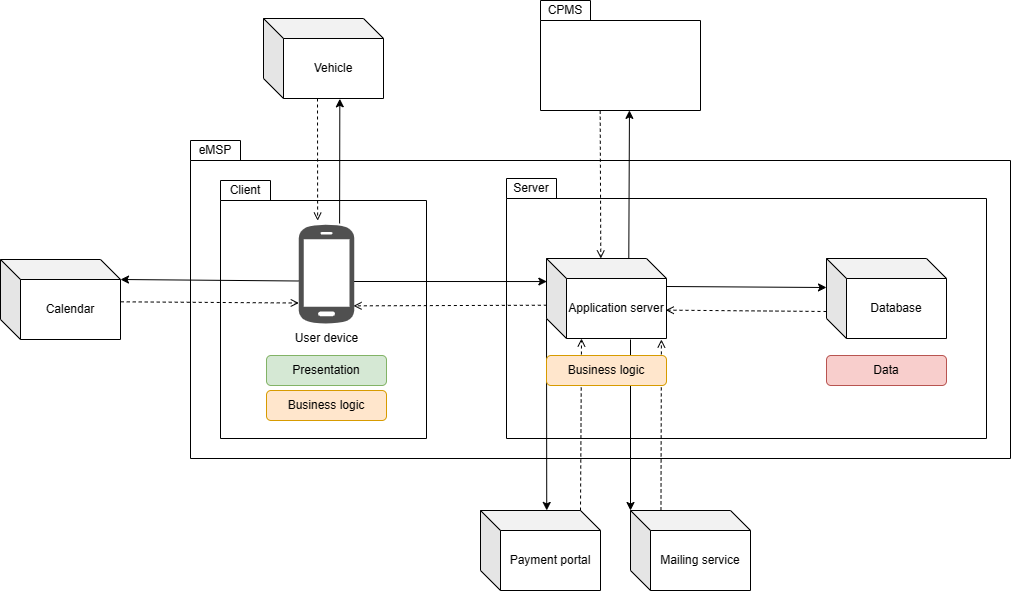
\includegraphics[keepaspectratio, width=0.75\textwidth]{Graphics/DD-eMSP-overview.drawio.png}
        \caption{\ac{eMSP} architectural overview}
        \label{fig:eMSP-overview-architecture}
    \end{center}
\end{figure}

The \ac{eMSP} is a \textbf{three-tier} architecture with \textbf{fat-clients} as seen in \autoref{fig:eMSP-overview-architecture}. This architecture is chosen for different reasons:
\begin{itemize}
    \item It makes the system more scalable;
    \item It allows the separation between business logic and data so that we can apply different levels of dependability to different decoupled systems and we can manage how data is accessed in a more granular way;
    \item A dedicated and optimized infrastructure (\ac{DBMS}) allows to handle a lot of data in the system (such as booked charges, all the infos about \acp{CPO}, \ldots);
    \item The database can only be accessible by the middleware, constituting an additional layer of security;
    \item With fat-clients the number of messages transmitted are fewer and lighter: an initial elaboration can be done on the smart devices of the user without sending a lot of raw data to the remote application server. The local on-the-edge elaboration is not considered as a problem given the computational power of smartphones.
\end{itemize}
The software pattern applied for this architecture is the \textbf{\ac{MVC} pattern}. This is best suited for our application because we want the components to be as modular, flexible and scalable as possible in order to simplify their distribution.

The following paragraphs will describe the principal components of this pattern and their architectural distribution.

\paragraph{Model}
The model is the logical representation of persistent data. This is stored in a database system and can only be directly accessed by the server application.

\paragraph{View}
The view logic is completely delegated to the client application, representing in different ways the data retrieved from the model (e.g. the charging stations sorting based on the user selected preferences).

\paragraph{Controller}
The controller has to manage all the client requests, interacting with the model, modifying it and returning to the view the changed/retrieved data.
For the most part, the business logic is in the server application. Retrieving and processing the vehicle and calendar data(in the case of a request for smart suggestions of the application) is handled by the client application to be as light as possible.

\subsubsection{\ac{CPMS} overview}

\begin{figure}[!h]
    \begin{center}
        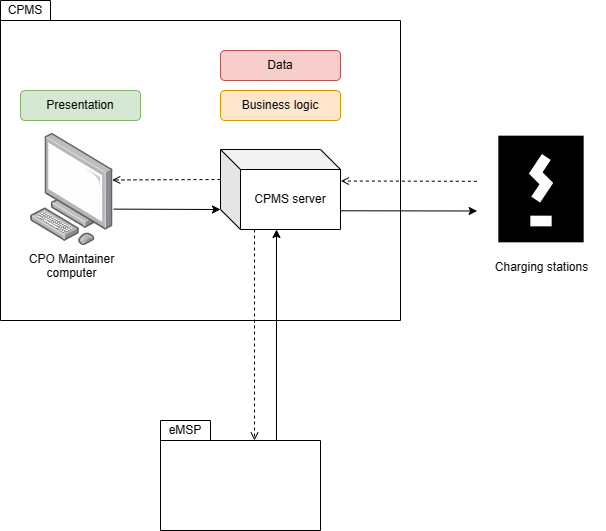
\includegraphics[keepaspectratio, width=0.75\textwidth]{Graphics/DD-CPMS-overview.drawio.png}
        \caption{\ac{CPMS} architectural overview}
        \label{fig:CPMS-overview-architecture}
    \end{center}
\end{figure}

The \ac{CPMS} follows the \textbf{two-tier} pattern with \textbf{thin-clients} as seen in \autoref{fig:CPMS-overview-architecture}. This architecture is chosen for different reasons:
\begin{itemize}
    \item The system is simpler to implement than the three-tier architecture;
    \item The system shouldn't handle so much data, thus it isn't necessary to have a dedicated architecture for the data layer;
    \item Clients are thin because they only have to view infos about charging stations and can send simple requests (for example \textit{use \ac{DSO} X for charging station Y}, \textit{set revenue percentage to Z}, etc.).
\end{itemize}
In this system the \ac{MVC} pattern is used. In this case, the client has only the view logic and can send simple requests. All the management of the \acp{DSO} and activation/deactivation of battery charging processes  are handled by the \ac{CPMS} server.
The \ac{CPMS} server deals also with charging requests from \acp{eMSP}, to which it responds with the elaborated data.

\subsection{Component view}
\begin{figure}[!h]
    \begin{center}
        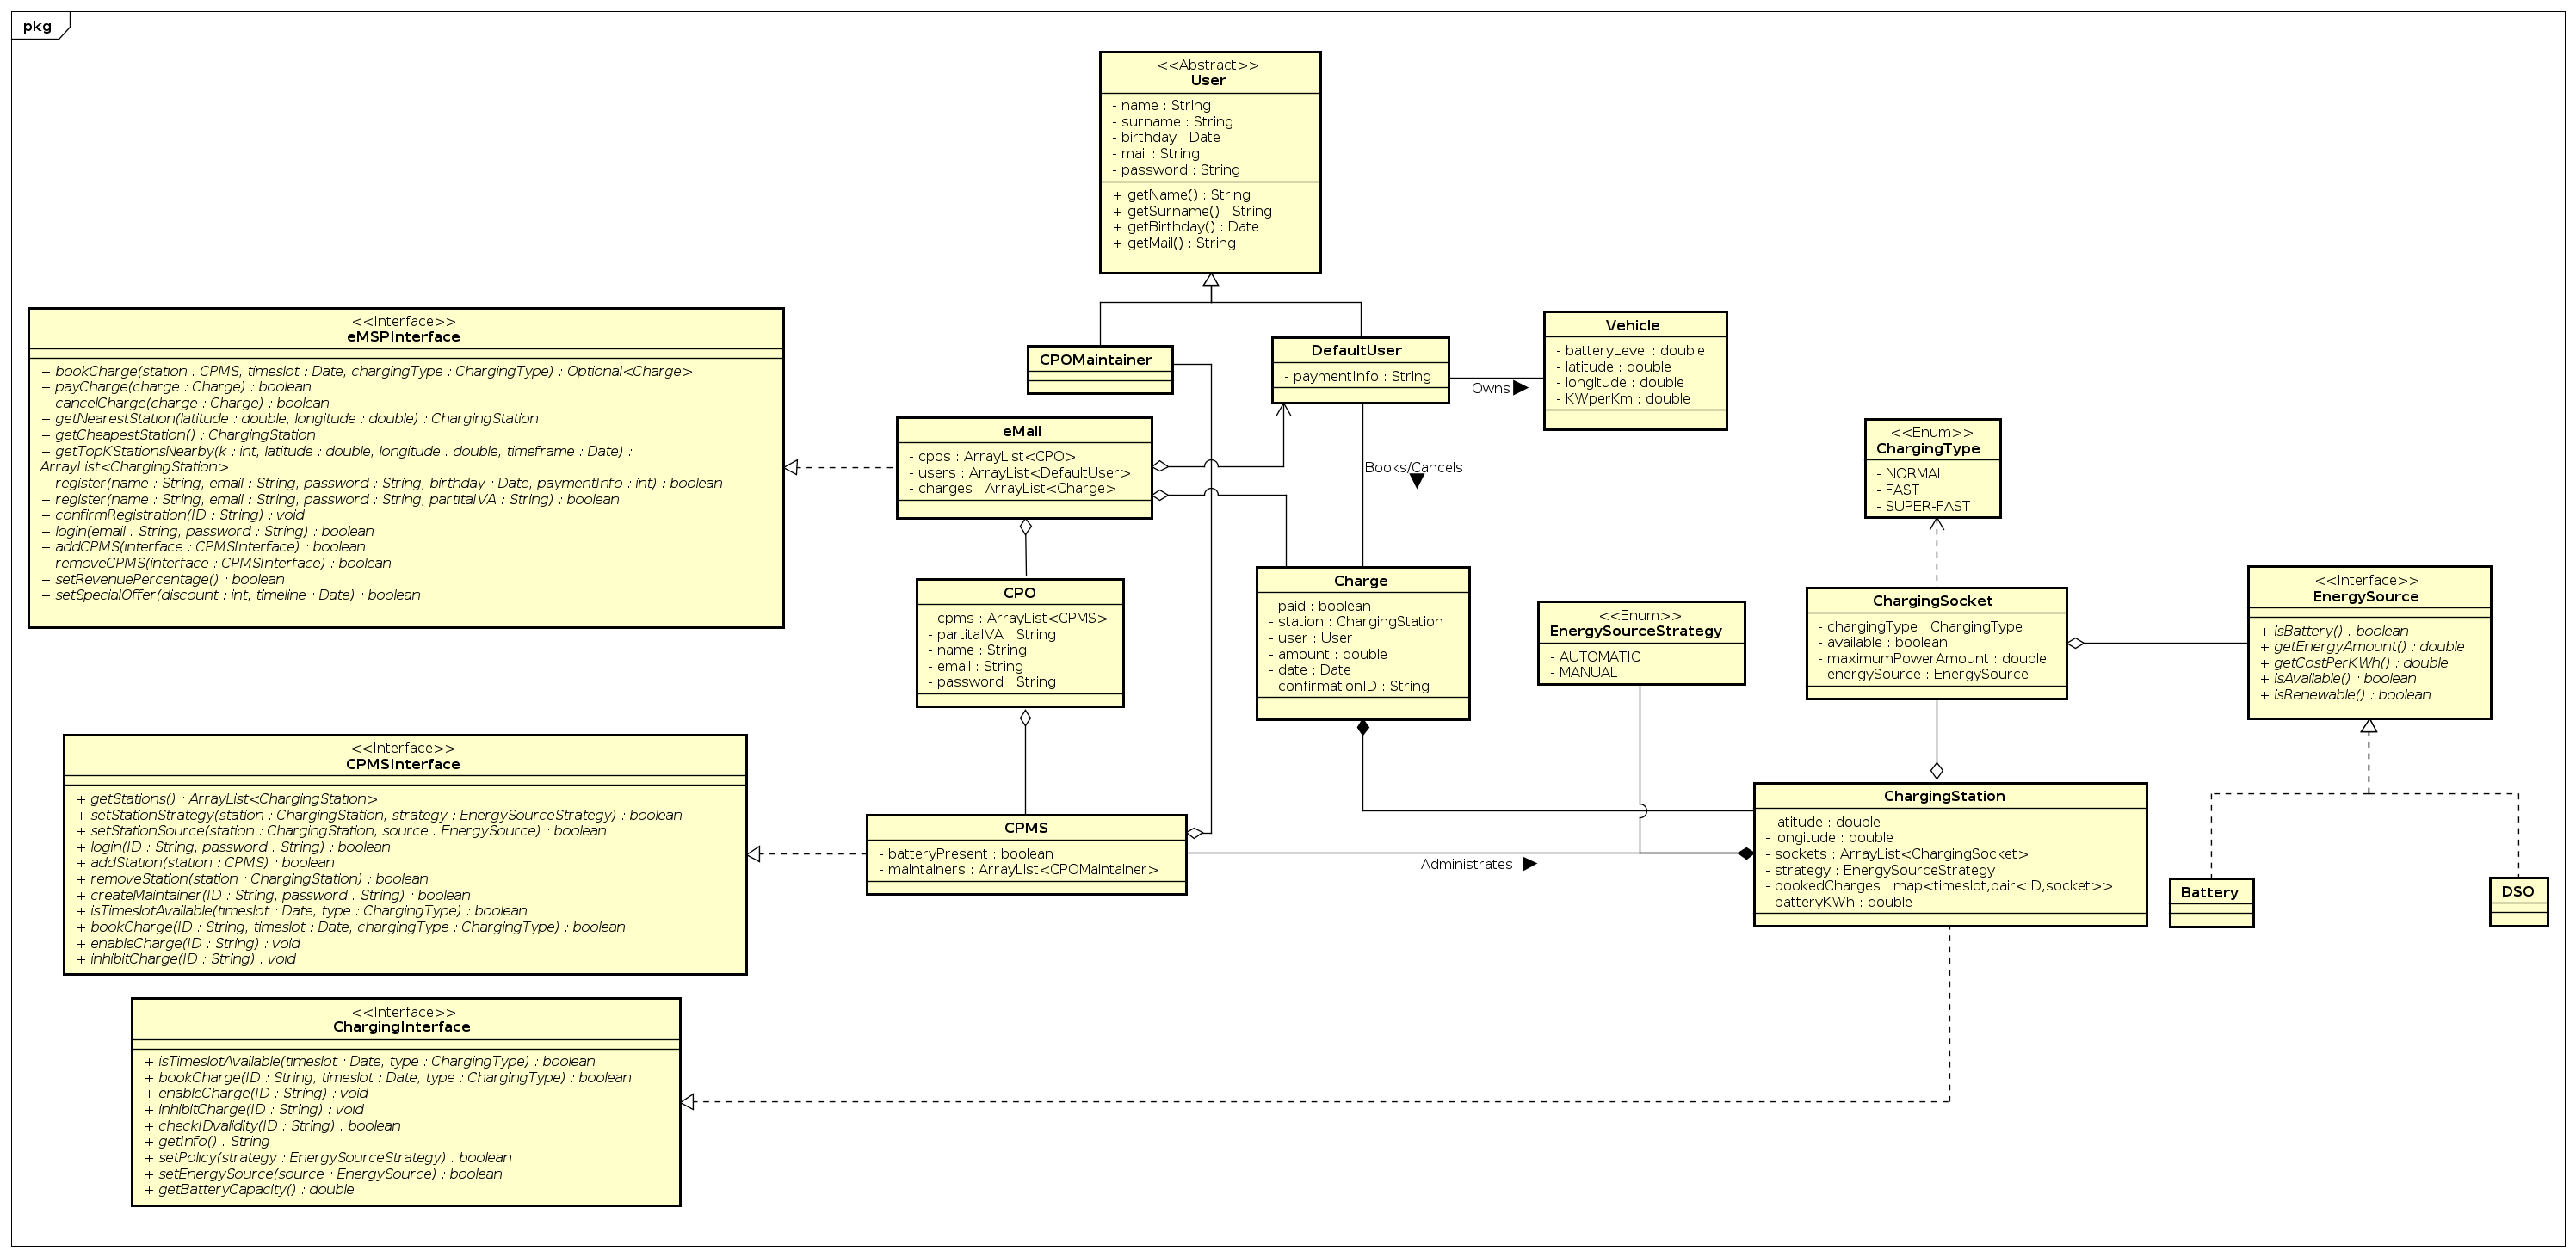
\includegraphics[keepaspectratio, width=16cm]{../RASD/RASD/UML.png}
        \caption{Class diagram}
        \label{fig:UML}
    \end{center}
\end{figure}
In the class diagram illustrated in \autoref{fig:UML} a model (not functional) view of the system is represented. The \ac{eMall} and \ac{CPMS} interfaces show what the two systems are expected to implement, whereas for the ChargingInterface and EnergySource it is assumed an already existing implementation.

\subsubsection{Component diagrams}
\begin{figure}[!h]
    \begin{center}
        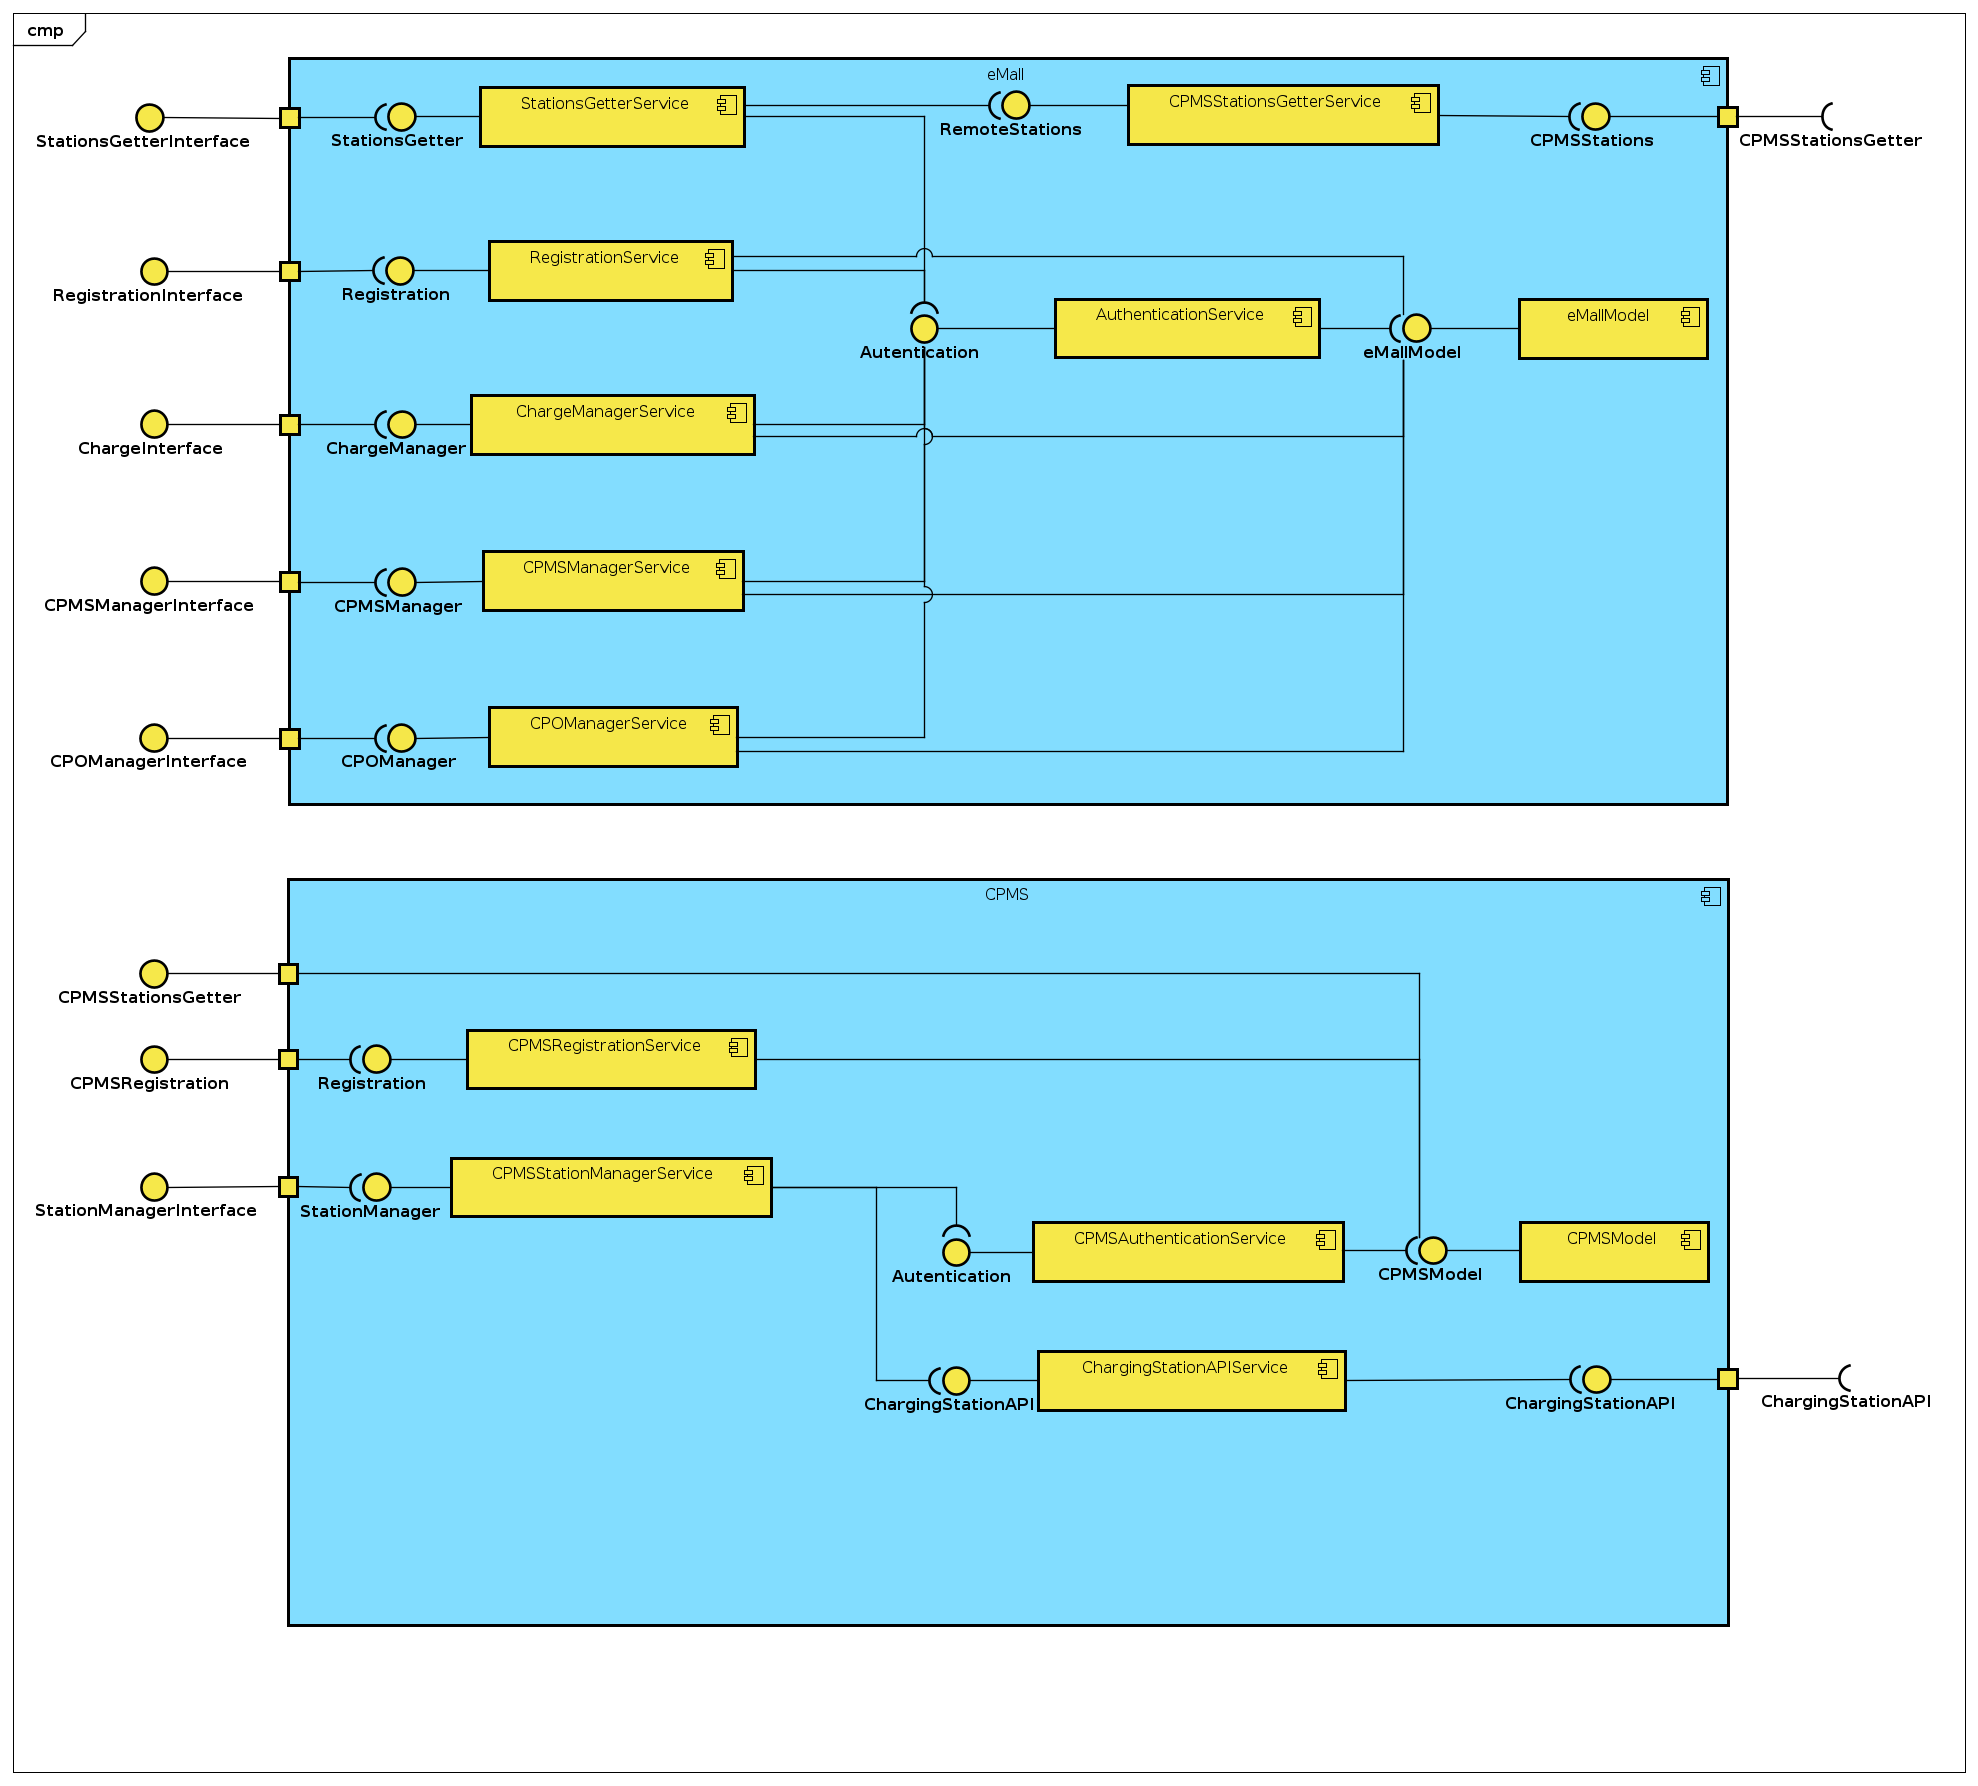
\includegraphics[keepaspectratio, width=16cm]{Component/Component.png}
        \caption{eMall component diagram}
        \label{fig:eMSP-component}
    \end{center}
\end{figure}
\clearpage
The two systems (\ac{eMall} and \ac{CPMS}) implement different interfaces and shows the \textit{Controller} and \textit{Model} parts of the \ac{MVC} pattern.
\makeatletter
\let\orgdescriptionlabel\descriptionlabel
\renewcommand*{\descriptionlabel}[1]{%
    \let\orglabel\label
    \let\label\@gobble
    \phantomsection
    \edef\@currentlabel{#1\unskip}%
    %\edef\@currentlabelname{#1}%
    \let\label\orglabel
    \orgdescriptionlabel{#1}%
}
\makeatother

\paragraph{\textbf{\ac{eMall}Client}}
The main components for the \ac{eMall}Client system are:
\begin{description}
    \item [\label{CalendarAPI}CalendarAPI] It is the component responsible for interfacing with a general web calendar in order to get the user's appointments;
    \item [\label{VehicleAPI}VehicleAPI] It is the component responsible for interfacing with a general electric vehicle in order to get vehicle infos;
    \item [\label{SuggestionEngine}SuggestionEngine] It is the component responsible for retrieving and parsing the data for a charge suggestion. It is the only active component of the \ac{eMall} system;
    \item [\label{eMallAPI}eMallAPI] It is the component in charge of remapping the client requests to the \ac{eMall} interface;
    \item [\label{eMallViewComponent}eMallViewComponent] It is the component in charge of handling the view logic and interfacing with the user through the \ac{UI};
\end{description}

\paragraph{\textbf{\ac{eMall}}}
The main components for the \ac{eMall} system are:
\begin{description}
    \item [\label{StationsComponent}StationsComponent] It is the component responsible for handling all the stations research requests (like \textit{getNearestStations}, \textit{getCheapestStation}, \textit{getTopKStationsNearby});
    \item [\label{RegistrationComponent}RegistrationComponent] It is the component responsible for handling the registration details along with the parameters checking during the registration phase;
    \item [\label{Timer}Timer] It is the component responsible for handling the registration verification timeout;
    \item [\label{ChargeManagerComponent}ChargeManagerComponent] It is the component responsible for handling all the charge booking/payment/cancellation processes. \\ It interfaces with the payment \ac{API} and with the \ref{CPMSAPI};
    \item [\label{CPMSManagerComponent}CPMSManagerComponent] It is the component responsible for handling the \ac{CPMS} operations from the \acp{CPO} users;
    \item [\label{CPOManagerComponent}CPOManagerComponent] It is the component responsible for handling the \acp{CPO} requests (like \textit{SetRevenuePercentage} and \textit{setSpecialOffer});
    \item [\label{CPMSAPI}CPMS API] It is the component responsible for interfacing the \ac{eMall} with the CPMS interfaces;
    \item [\label{AuthenticationComponent}AuthenticationComponent] It is the component responsible for authorizing every operation. In this component it is implemented part of the controller (of the \ac{MVC} pattern) to check if an operation is legit for the account type;
    \item [\label{MailAPI}Mail API] It is the component responsible for sending the feedback emails to the user every time an important operation is done;
    \item [\label{PaymentAPI}Payment API] It is the component responsible for performing financial operations/verifications;
    \item [\label{eMallModel}eMall Model] It is the core model component. It interfaces the \ac{DBMS} with the rest of system components.
\end{description}
\clearpage
\paragraph{\textbf{\ac{CPMS}}}
The main components for the \ac{CPMS} system are:
\begin{description}
    \item [\label{CPMSRegistrationComponent}CPMSRegistrationComponent] It is the component responsible for handling the registration details of new \ac{CPO} maintainers;
    \item [\label{CPMSStationManagerComponent}CPMSStationManagerComponent] It is the component responsible for handling all the station managing actions from a \ac{CPO} maintainer (\textit{setStationStrategy}, \textit{setStationSource}..);
    \item [\label{CPMSChargeManagerComponent}CPMSChargeManagerComponent] It is the component responsible for handling all the actions which involve book/enable/inhibit a charge. The \ac{eMall} is the only component that utilizes this interface;
    \item [\label{CPMSAuthenticationComponent}CPMSAuthenticationComponent] It is the component responsible for authorizing every operation. In this component it is implemented part of the controller (of the \ac{MVC} pattern) to check if an operation is legit;
    \item [\label{CPMSChargingStationAPI}CPMSChargingStation API] It is the component that interfaces the \ac{CPMS} system with the external Charging Stations;
    \item [\label{CPMSModel}CPMSModel] It is the core component. It stores all the \ac{CPMS} data and interfaces them with the other system components.
\end{description}
In the component diagrams, there are components (\textit{Payment\ac{API}}, \textit{\ac{CPMS}\ac{API}}, \textit{Mail\ac{API}}, \\\textit{\ac{CPMS}ChargingStationAPI}) that could be bypassed, letting the main components interface the external \acp{API}. These components are integrated because they offer the possibility to contain the external interface standards in one single component. This creates the possibility for developers to create an internal interfacing standard different from the external ones.

\subsection{Deployment view}
The general idea of the deployment view is to show all the main architectural components with the distribution of the artifacts (applications, firewall rule tables, data\ldots).

\subsubsection{\ac{eMSP}}
\begin{figure}[!h]
    \begin{center}
        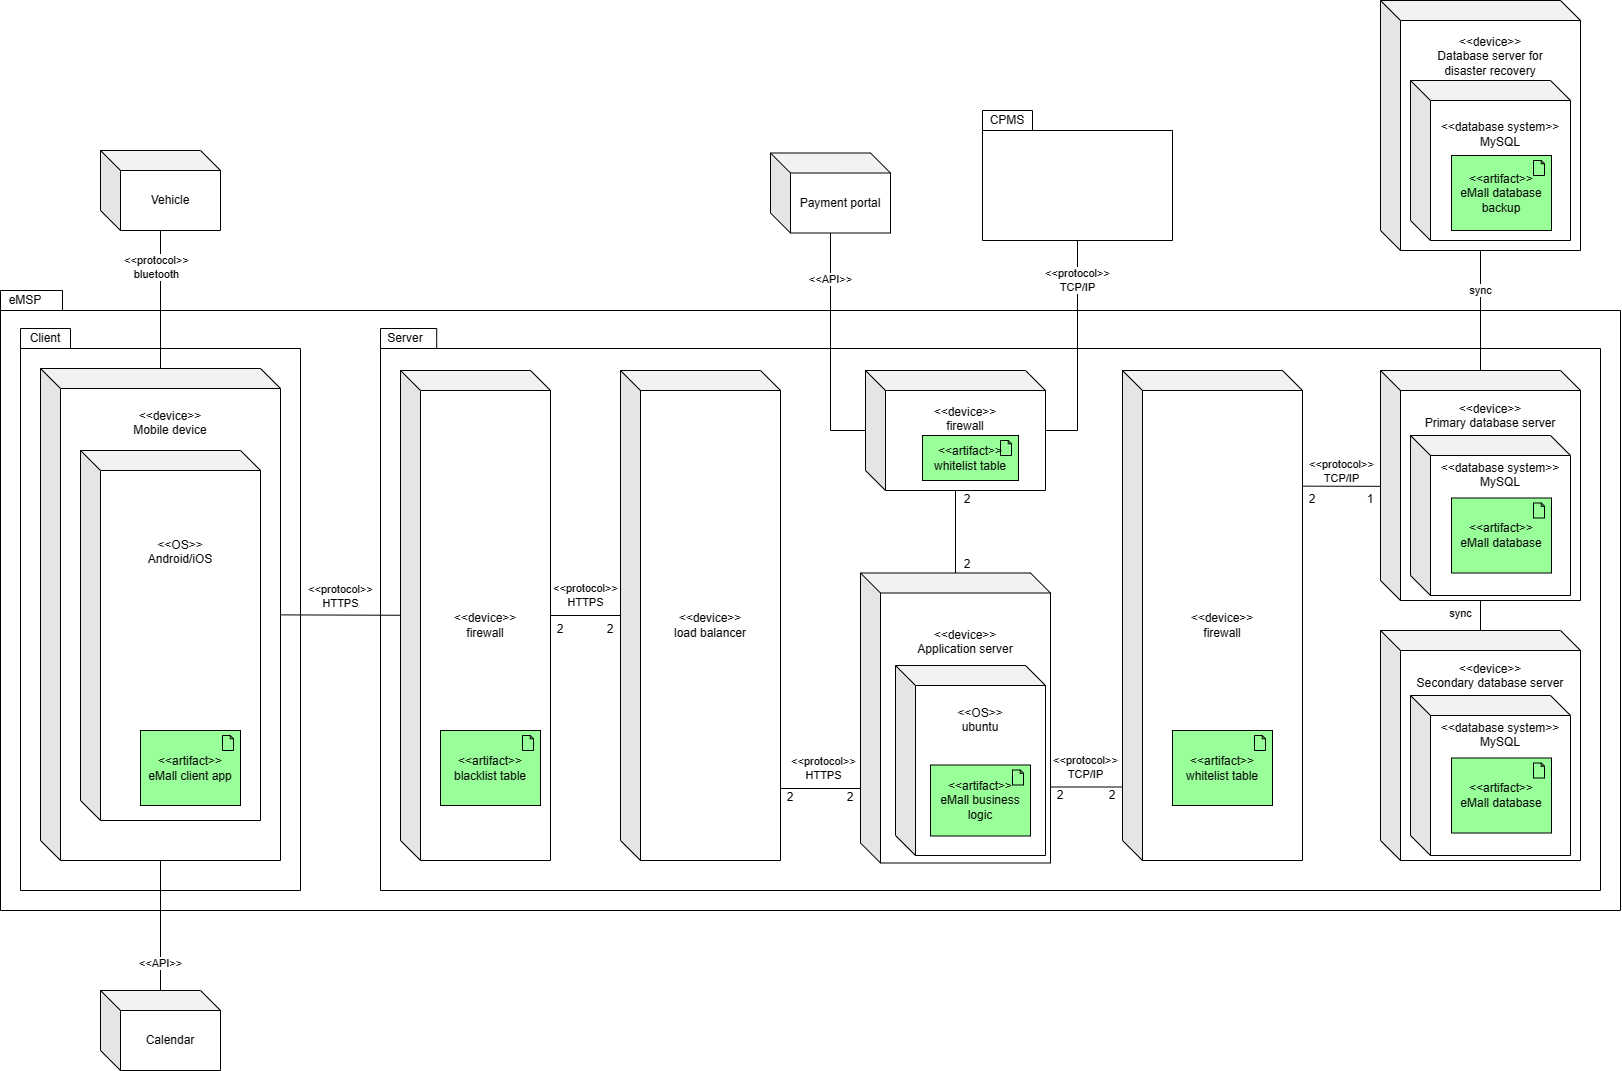
\includegraphics[keepaspectratio, width=0.9\textwidth]{Graphics/DD-eMSP-deployment.drawio.png}
        \caption{eMall deployment view diagram}
        \label{fig:eMSP-deployment}
    \end{center}
\end{figure}

The system has been designed to provide security policies and avoid \acp{SPOF}, to support an high availability service. The system's components are:
\begin{itemize}
    \item Mobile device: It is the device used by users or \acp{CPO} to interact with the \ac{eMall} system. It is provided with internet connection, bluetooth peripheral and the \ac{eMall} client application installed. This application must be available for both Android and iOS mobile operative systems in order to be compatible with most devices.
          It uses \ac{HTTPS} to communicate with the server and the calendar. \ac{HTTPS} provides different security layers and it is compliant with the \ac{GDPR} law. The device uses bluetooth to create a \ac{PAN} with the user's vehicle to retrieve its data.
    \item Application server: The physical server that runs the \ac{eMSP} application, which receives all the requests from the clients and hosts the business logic. There are two redundant application servers in order to increase reliability and availability avoiding down-times while maintaining the \ac{eMall} service.
          Ubuntu is chosen as the server's Operative System because; it is open source and the most used linux distribution according to \cite{ref:most-popular-linux-distro}. Thus support and compatibility is assured by its widespread usage.
    \item Load balancer: balances the load of the requests among the active application servers and it handles server failures. This system provides failover as described in \\\cite{ref:redundant-load-balancers}.
    \item Firewall: Each firewall in the server is used to isolate different zones. A first firewall interfaces the external world to the load balancer in order to filter dangerous requests.
          A blacklist rule table is implemented due to the difficulties with an allowlist. For the internal firewall an allowlist table is implemented to enable only application servers communications with databases. This system provides failover as described in \cite{ref:redundant-firewalls}.
    \item Database system: A redundant database system is deployed. The secondary database should always be synchronized with the primary one in order to be ready for an eventual substitution in case of failure as described in \cite{ref:redundant-databases}. A disaster recovery database is also necessary. MySQL \ac{DBMS} has been chosen because it is one of the most used as stated in \cite{ref:most-popular-RDBMS}.
\end{itemize}

\subsubsection{\ac{CPMS}}
\begin{figure}[!h]
    \begin{center}
        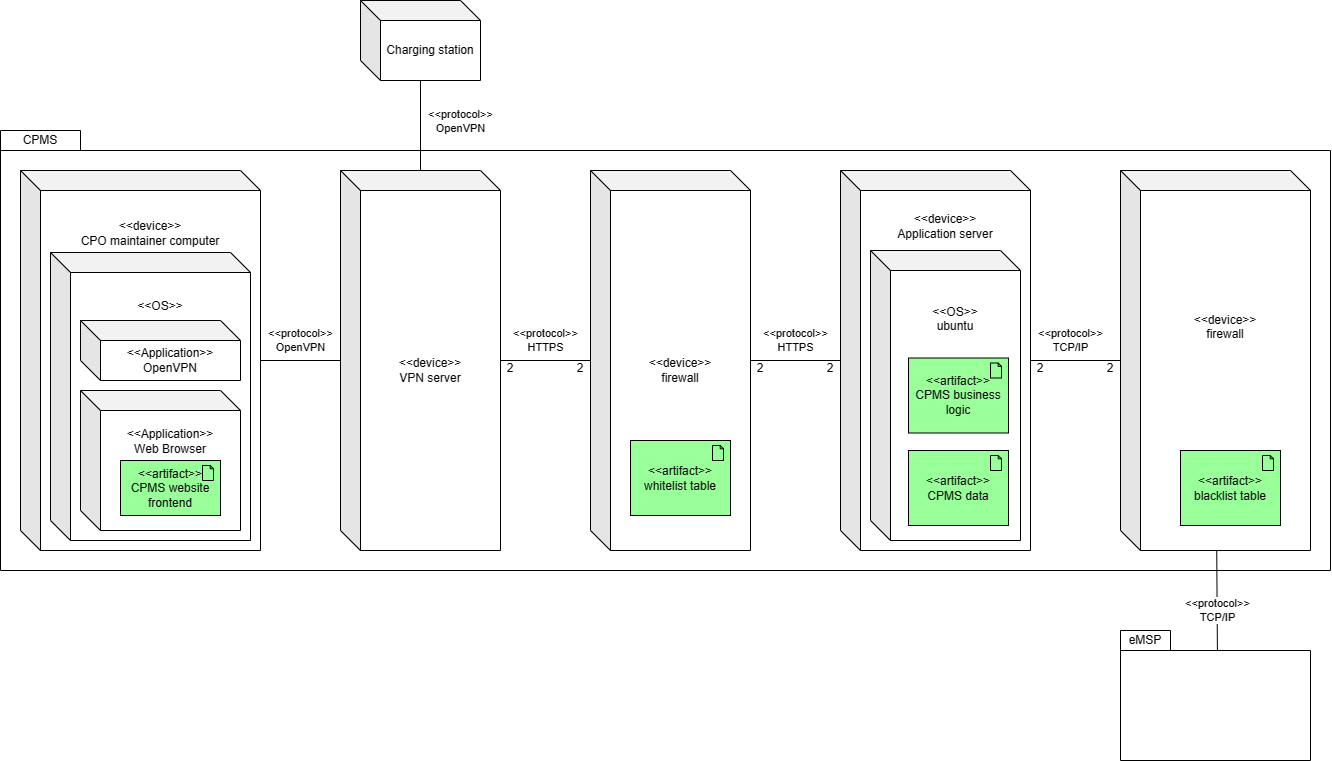
\includegraphics[keepaspectratio, width=0.9\textwidth]{Graphics/DD-CPMS-deployment.drawio.png}
        \caption{CPMS deployment view diagram}
        \label{fig:CPMS-deployment}
    \end{center}
\end{figure}

In the \ac{CPMS} a \ac{VPN} is implemented so that only \ac{CPO}maintainers in the same \ac{VPN} have the ability to perform actions. The only non-\ac{VPN} connections come from \acp{eMSP}.
Redundancy is implemented in order to avoid \acp{SPOF}.
The system components are:
\begin{itemize}
    \item \ac{CPO} maintainer computer: This device is connected through a \ac{VPN} to a \ac{VPN} server. It can connect to the \ac{CPMS} site with a web browser on top of an Operative System.
          This is the thin client, the \ac{CPMS}' website front-end just handles the view and sends requests to the application server.
    \item \ac{VPN} server: It allows the \ac{CPO} maintainer computers, the charging stations and the application server to share the same private network to simplify the communication and improve the overall security.
          The OpenVPN protocol \cite{ref:openvpn-site} has been chosen because it is an open source project. It is considered a secure protocol and it is widely used in many different applications.
          This system provides failover as described in \cite{ref:redundant-VPN-servers}.
    \item Application server: This is the component that handles all the requests to the system and redirects them to the charging stations if needed. This system is redundant in order to assure availability during maintenance.
          Ubuntu is chosen as the server's Operative System because; it is open source and the most used linux distribution according to \cite{ref:most-popular-linux-distro}. Thus support and compatibility is assured by its widespread usage.
    \item Firewalls: They encapsulate the application server to enforce security policies. The system provides failover as described in \cite{ref:redundant-firewalls}.
\end{itemize}
\clearpage

\subsection{Runtime view}
\begin{figure}[!h]
    \begin{center}
        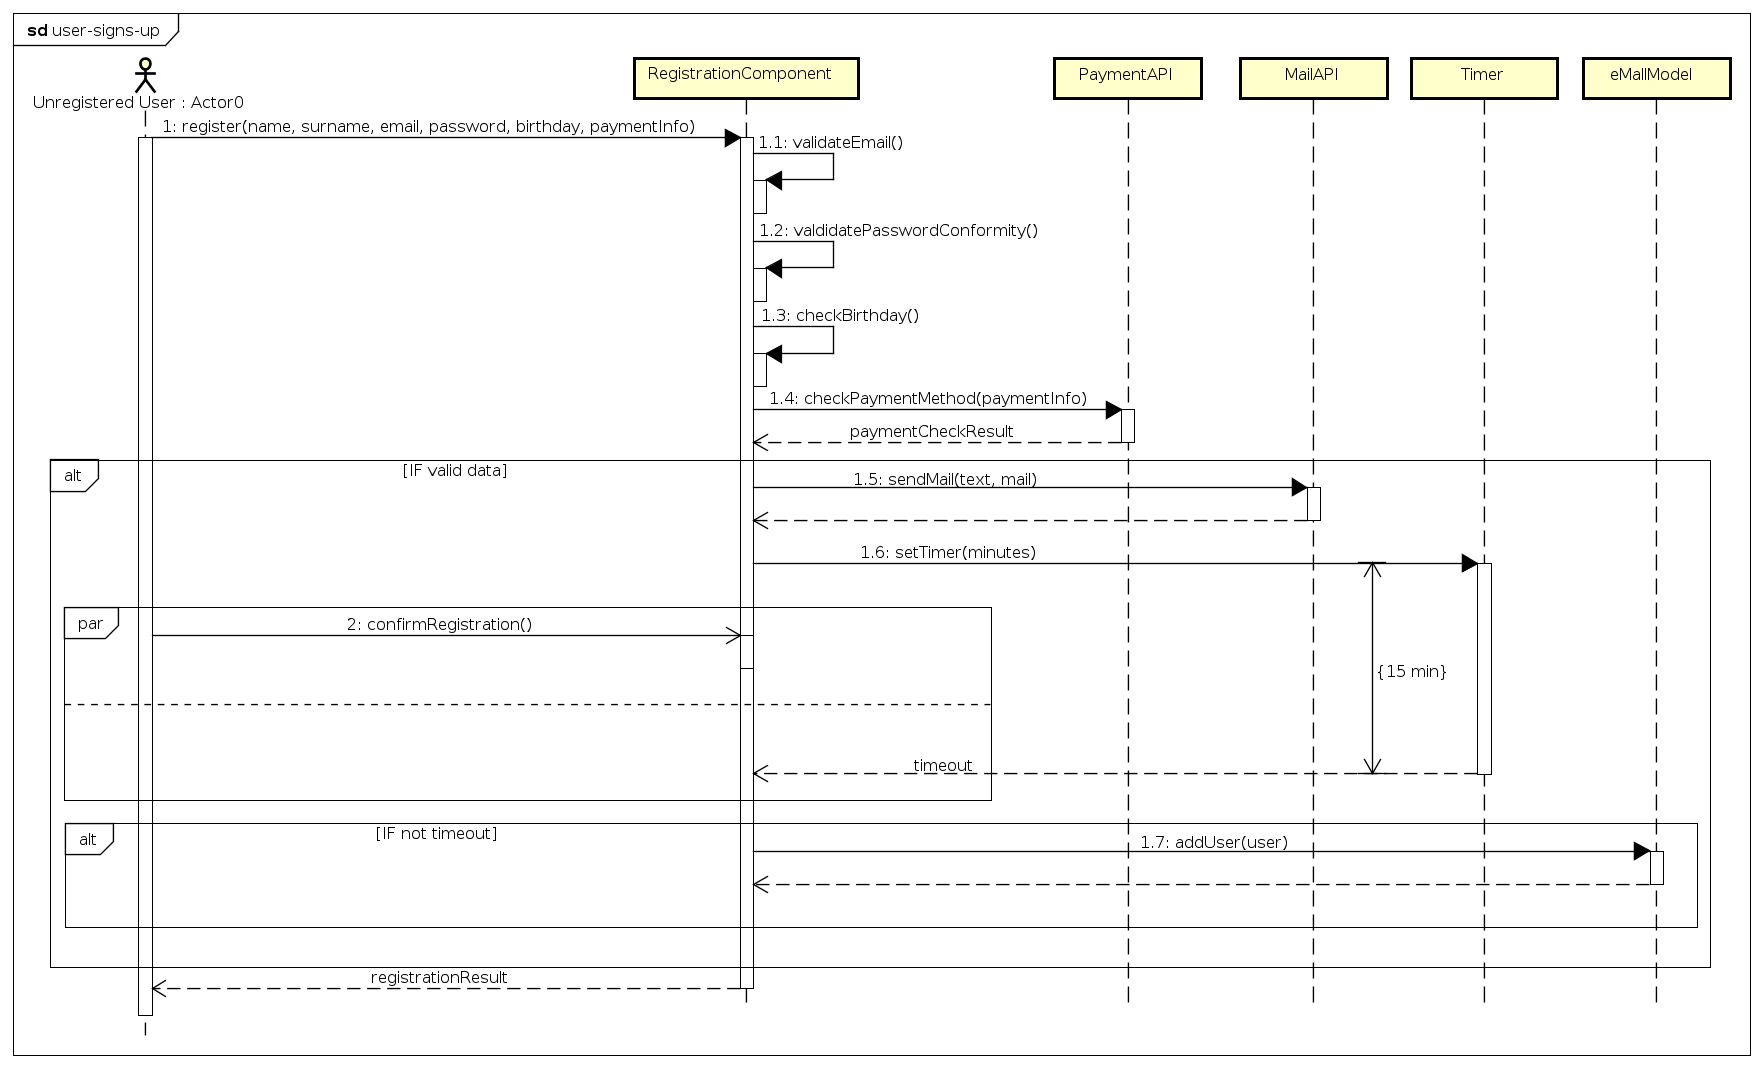
\includegraphics[keepaspectratio, width=16cm]{Sequence/user-signs-up.png}
        \caption{User signs up}
        \label{fig:user-signs-up}
    \end{center}
\end{figure}
\begin{figure}[!h]
    \begin{center}
        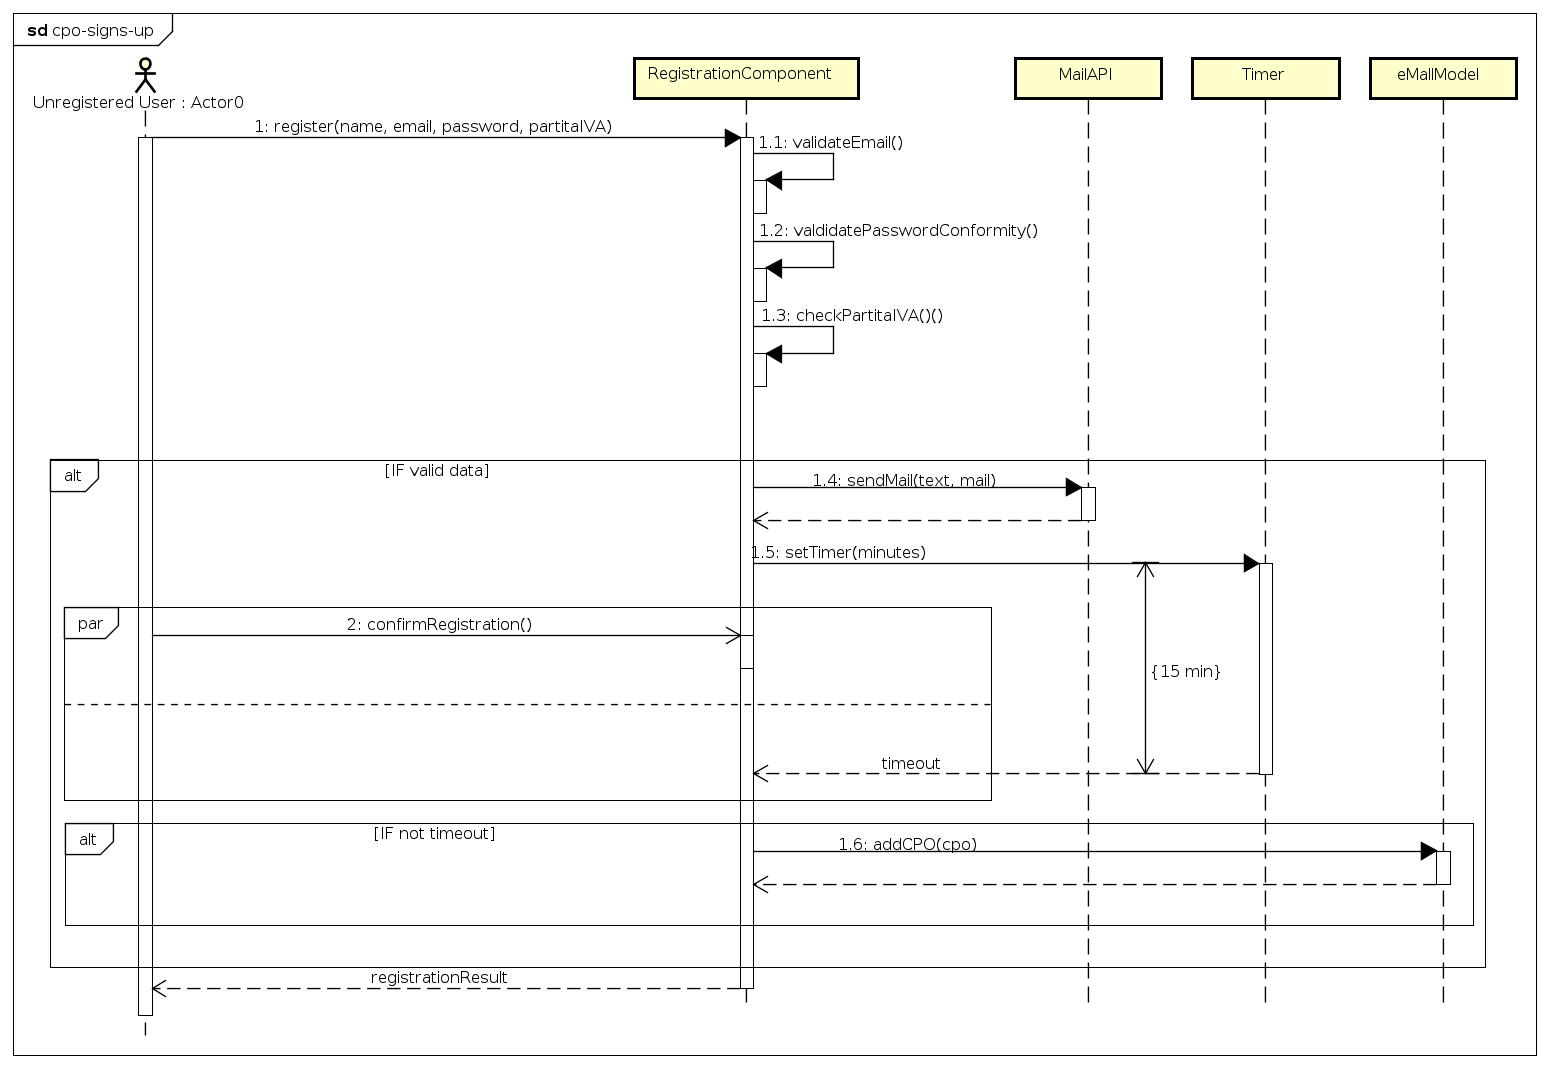
\includegraphics[keepaspectratio, width=16cm]{Sequence/cpo-signs-up.png}
        \caption{\ac{CPO} signs up}
        \label{fig:cpo-signs-up}
    \end{center}
\end{figure}
\begin{figure}[!h]
    \begin{center}
        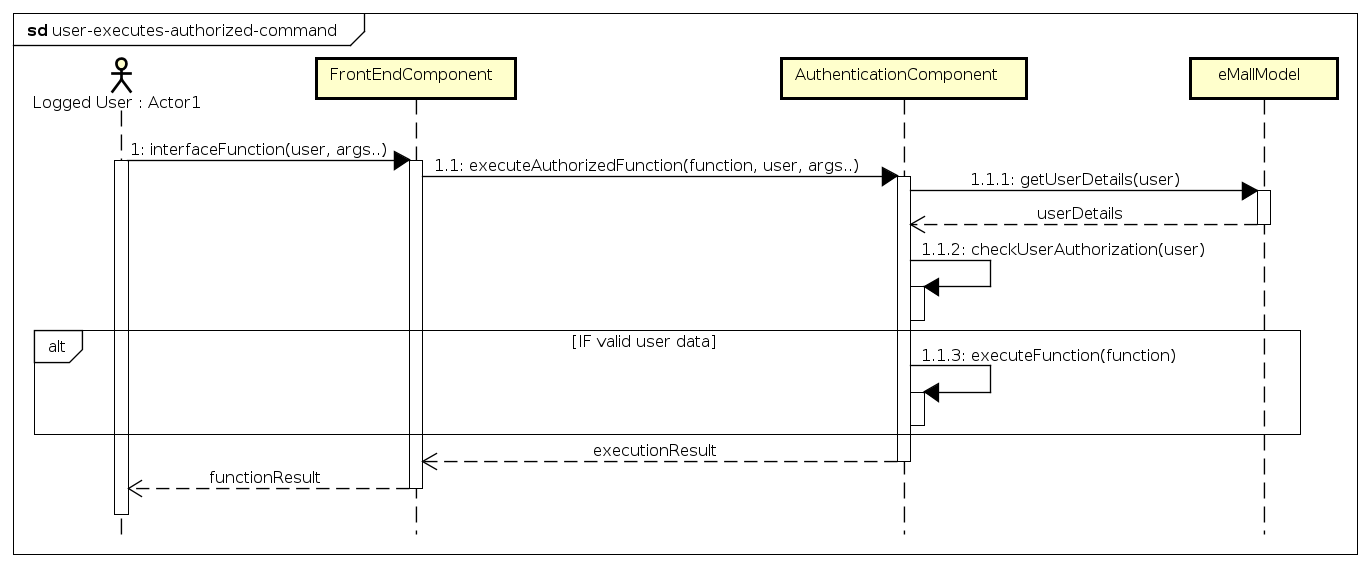
\includegraphics[keepaspectratio, width=16cm]{Sequence/user-executes-authorized-command.png}
        \caption{User executes authorized command}
        \label{fig:user-executes-authorized-command}
    \end{center}
\end{figure}
\begin{figure}[!h]
    \begin{center}
        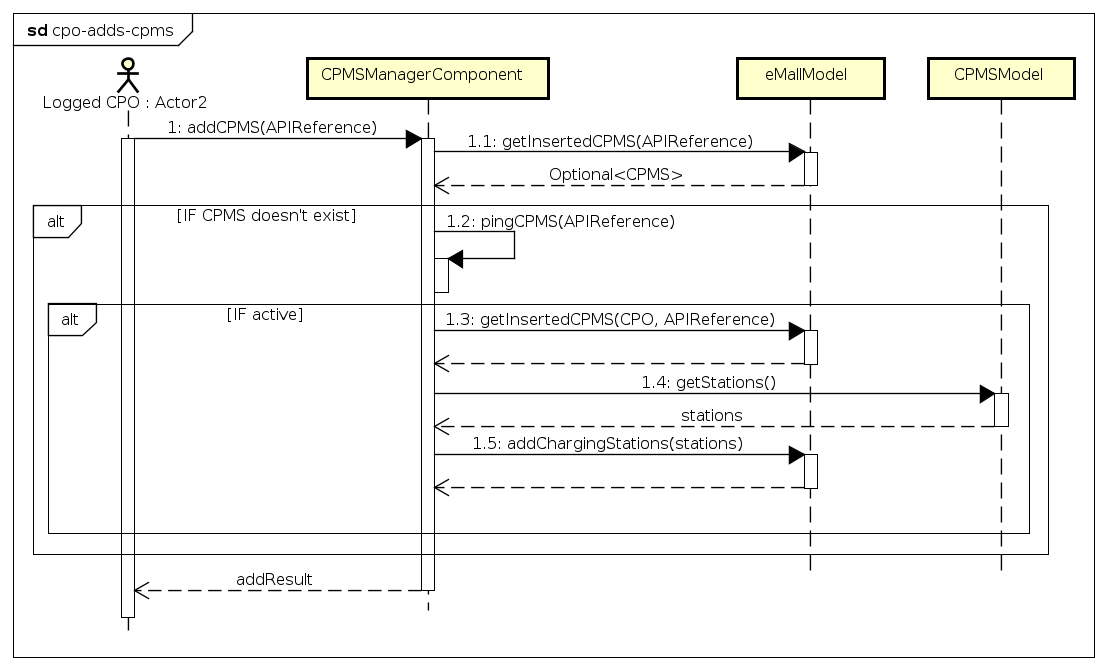
\includegraphics[keepaspectratio, width=16cm]{Sequence/cpo-adds-cpms.png}
        \caption{\ac{CPO} adds \ac{CPMS} into \ac{eMall}}
        \label{fig:cpo-adds-cpms}
    \end{center}
\end{figure}
\begin{figure}[!h]
    \begin{center}
        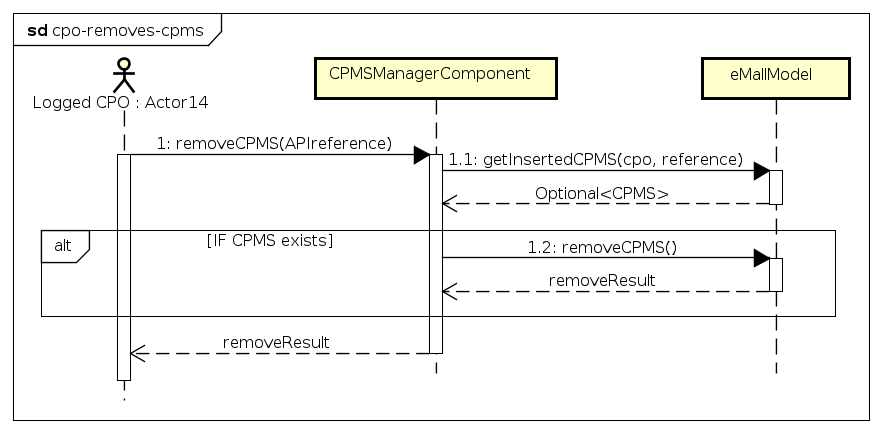
\includegraphics[keepaspectratio, width=16cm]{Sequence/cpo-removes-cpms.png}
        \caption{\ac{CPO} removes \ac{CPMS} from \ac{eMall}}
        \label{fig:cpo-removes-cpms}
    \end{center}
\end{figure}
\begin{figure}[!h]
    \begin{center}
        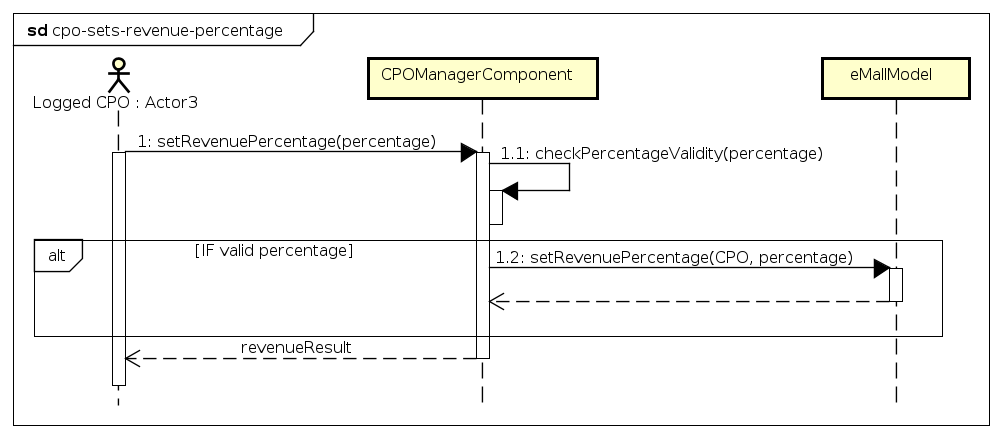
\includegraphics[keepaspectratio, width=16cm]{Sequence/cpo-sets-revenue-percentage.png}
        \caption{\ac{CPO} sets the revenue percentage}
        \label{fig:cpo-sets-revenue-percentage}
    \end{center}
\end{figure}
\begin{figure}[!h]
    \begin{center}
        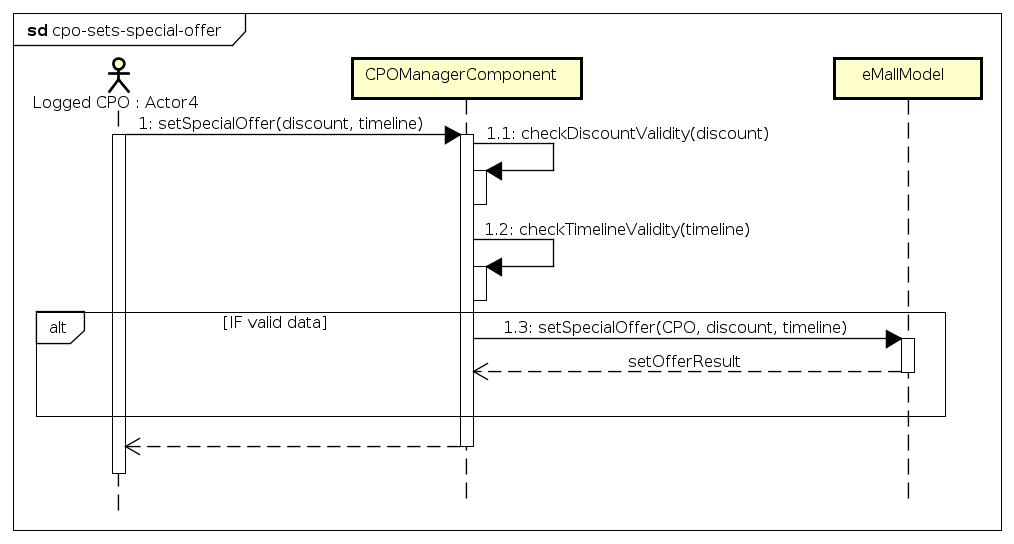
\includegraphics[keepaspectratio, width=16cm]{Sequence/cpo-sets-special-offer.png}
        \caption{\ac{CPO} sets a special offer}
        \label{fig:cpo-sets-speciale-offer}
    \end{center}
\end{figure}
\begin{figure}[!h]
    \begin{center}
        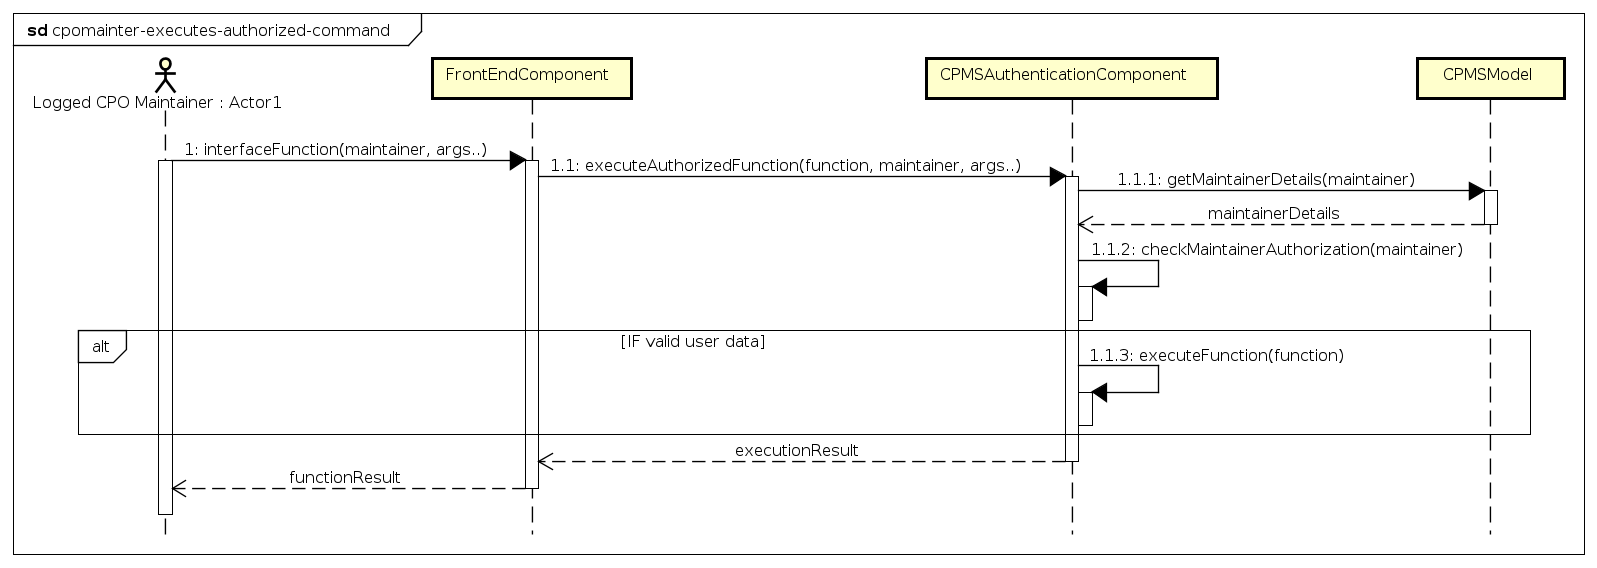
\includegraphics[keepaspectratio, width=16cm]{Sequence/cpomaintainer-executes-authorized-command.png}
        \caption{\ac{CPO}maintainer executes authorized command}
        \label{fig:cpomaintainer-executes-authorized-command}
    \end{center}
\end{figure}
\begin{figure}[!h]
    \begin{center}
        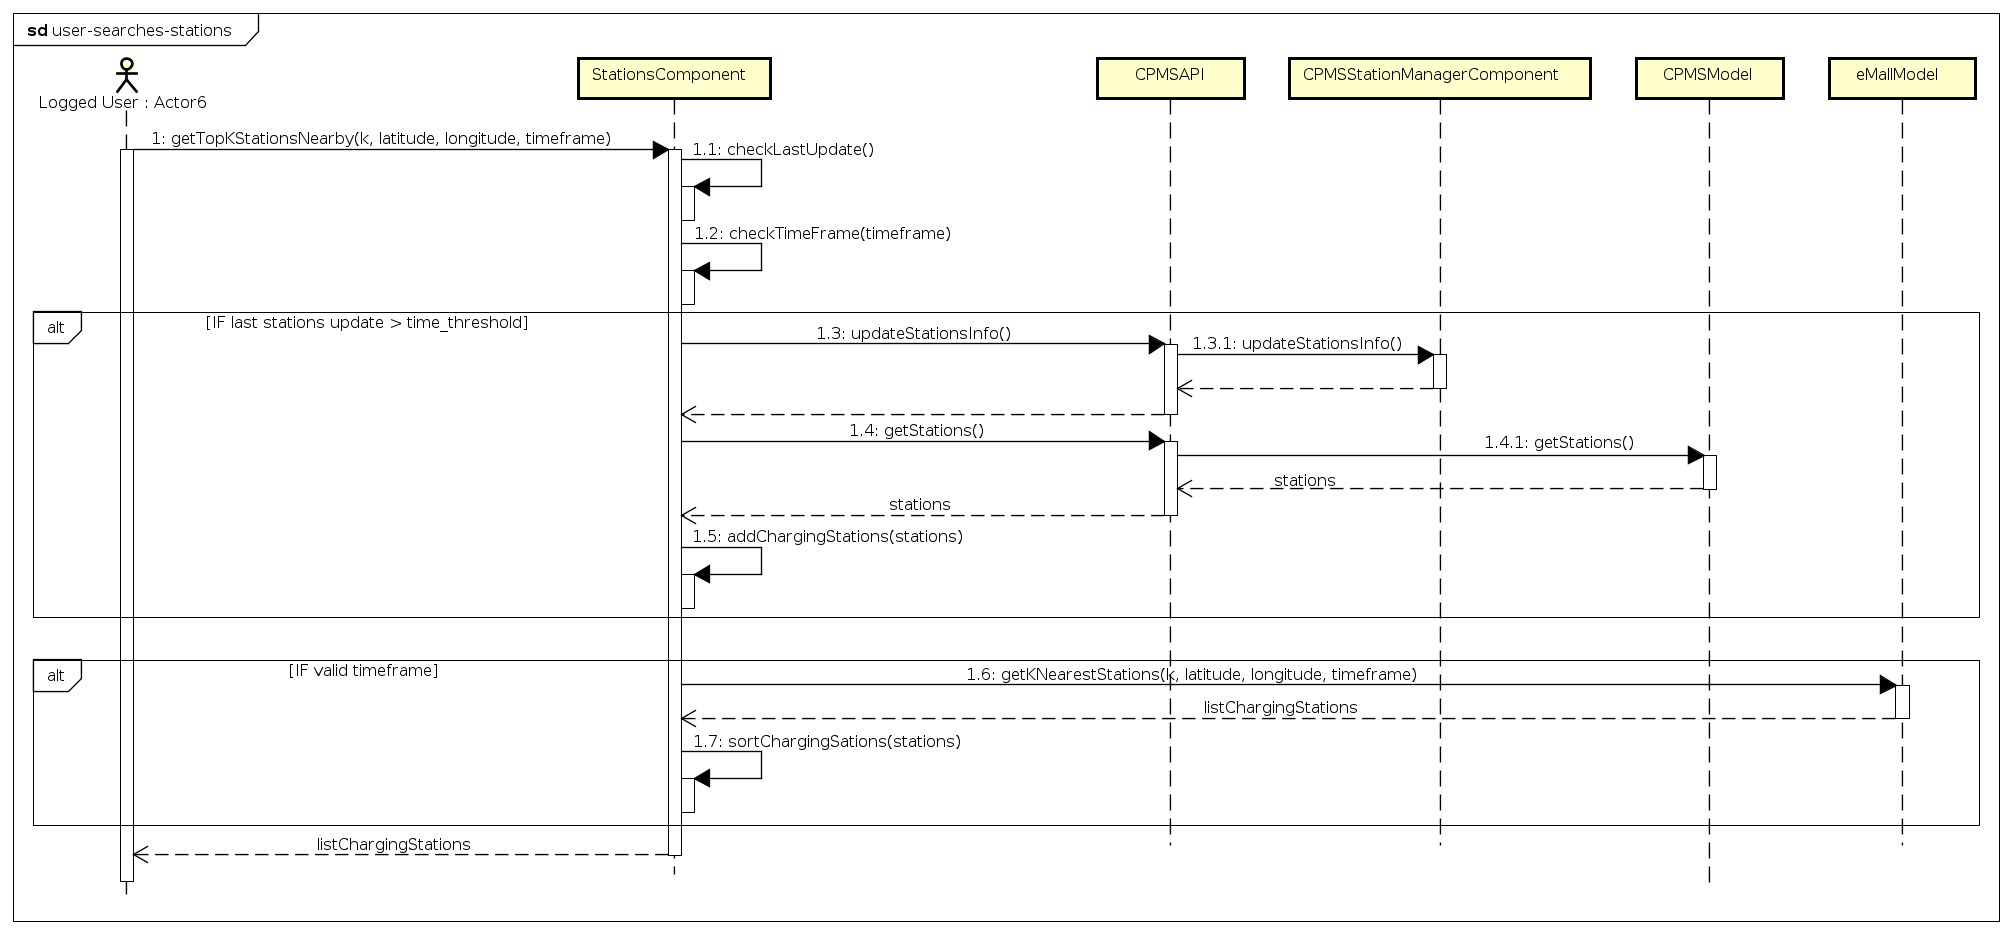
\includegraphics[keepaspectratio, width=16cm]{Sequence/user-searches-stations.png}
        \caption{Get the nearby charging stations}
        \label{fig:user-searches-stations}
    \end{center}
\end{figure}
\begin{figure}[!h]
    \begin{center}
        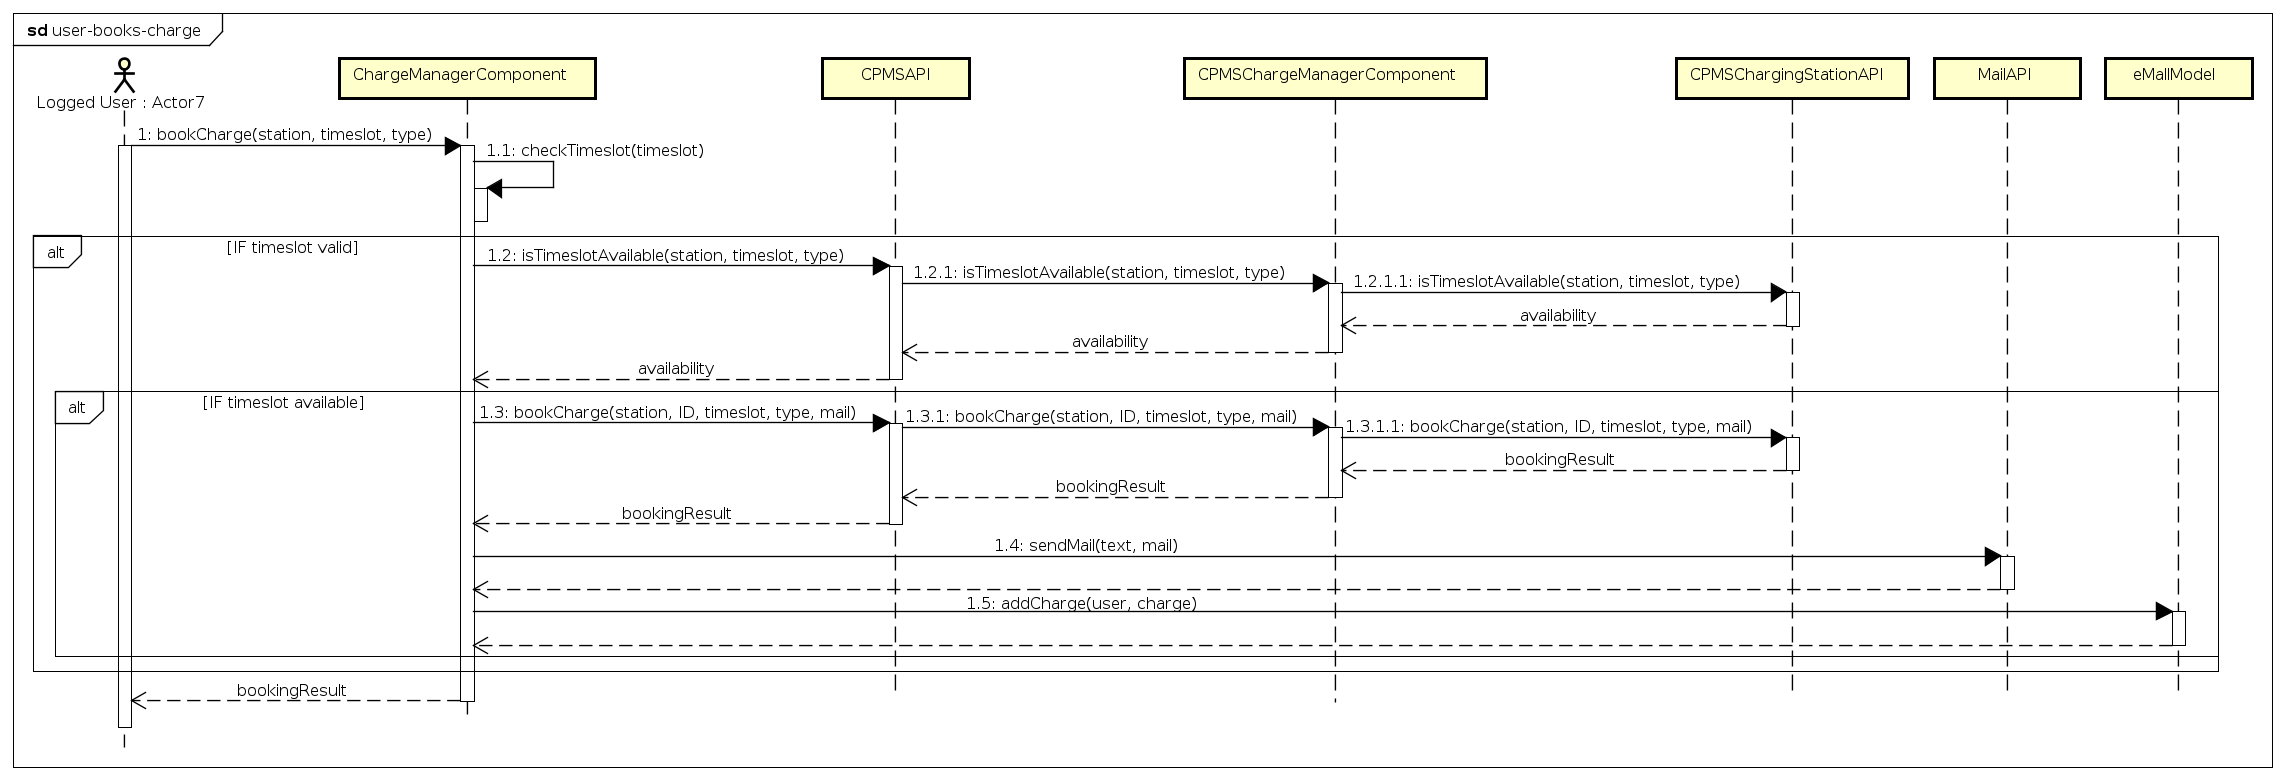
\includegraphics[keepaspectratio, width=16cm]{Sequence/user-books-charge.png}
        \caption{Book a charge sequence}
        \label{fig:user-books-charge}
    \end{center}
\end{figure}
\begin{figure}[!h]
    \begin{center}
        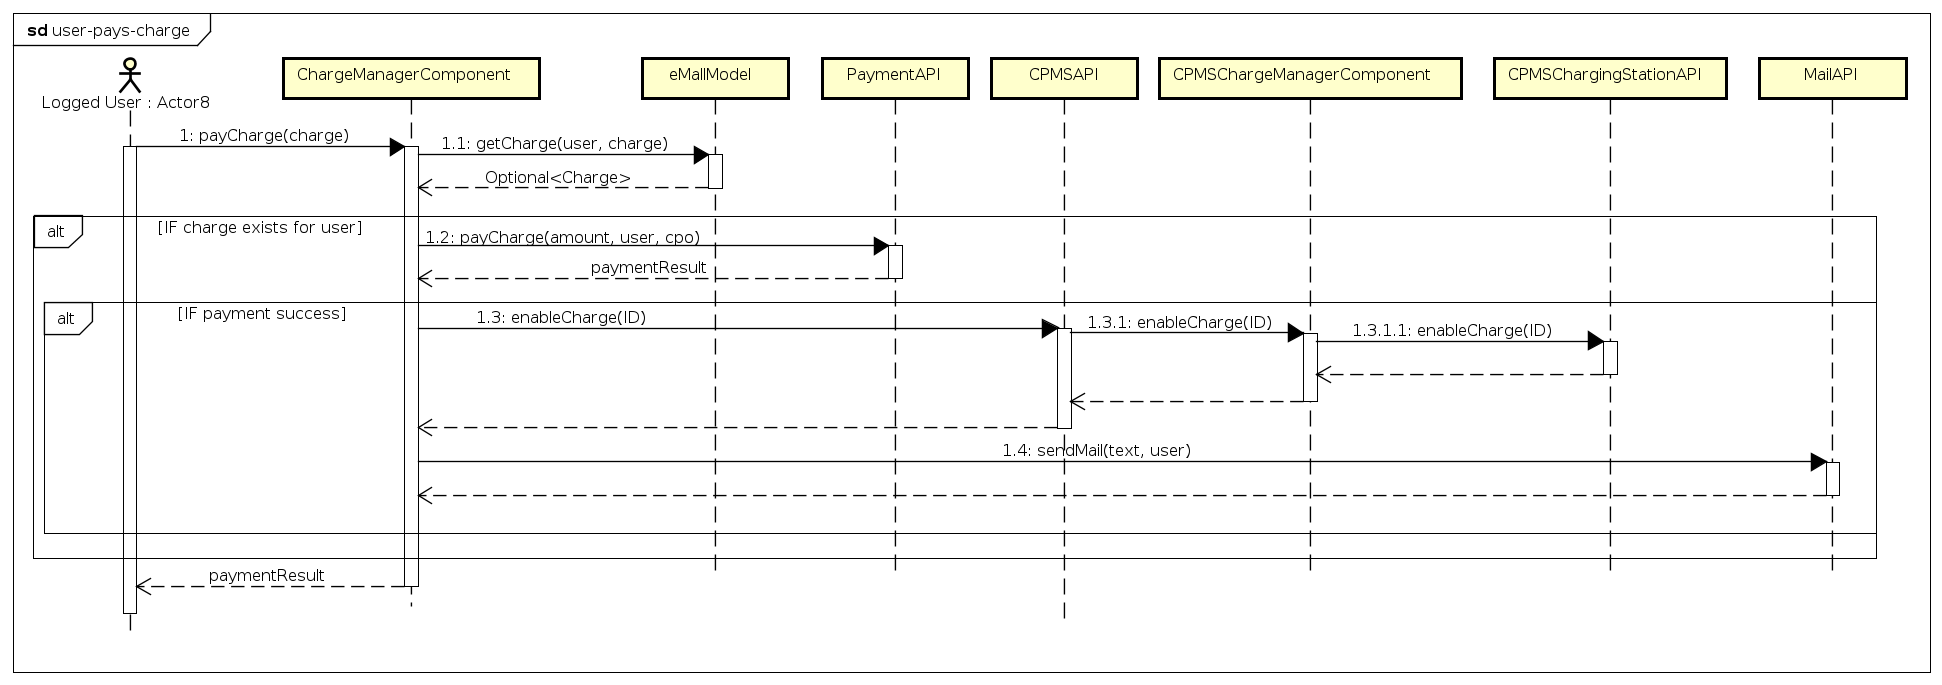
\includegraphics[keepaspectratio, width=16cm]{Sequence/user-pays-charge.png}
        \caption{Pay a charge sequence}
        \label{fig:user-pays-charge}
    \end{center}
\end{figure}
\begin{figure}[!h]
    \begin{center}
        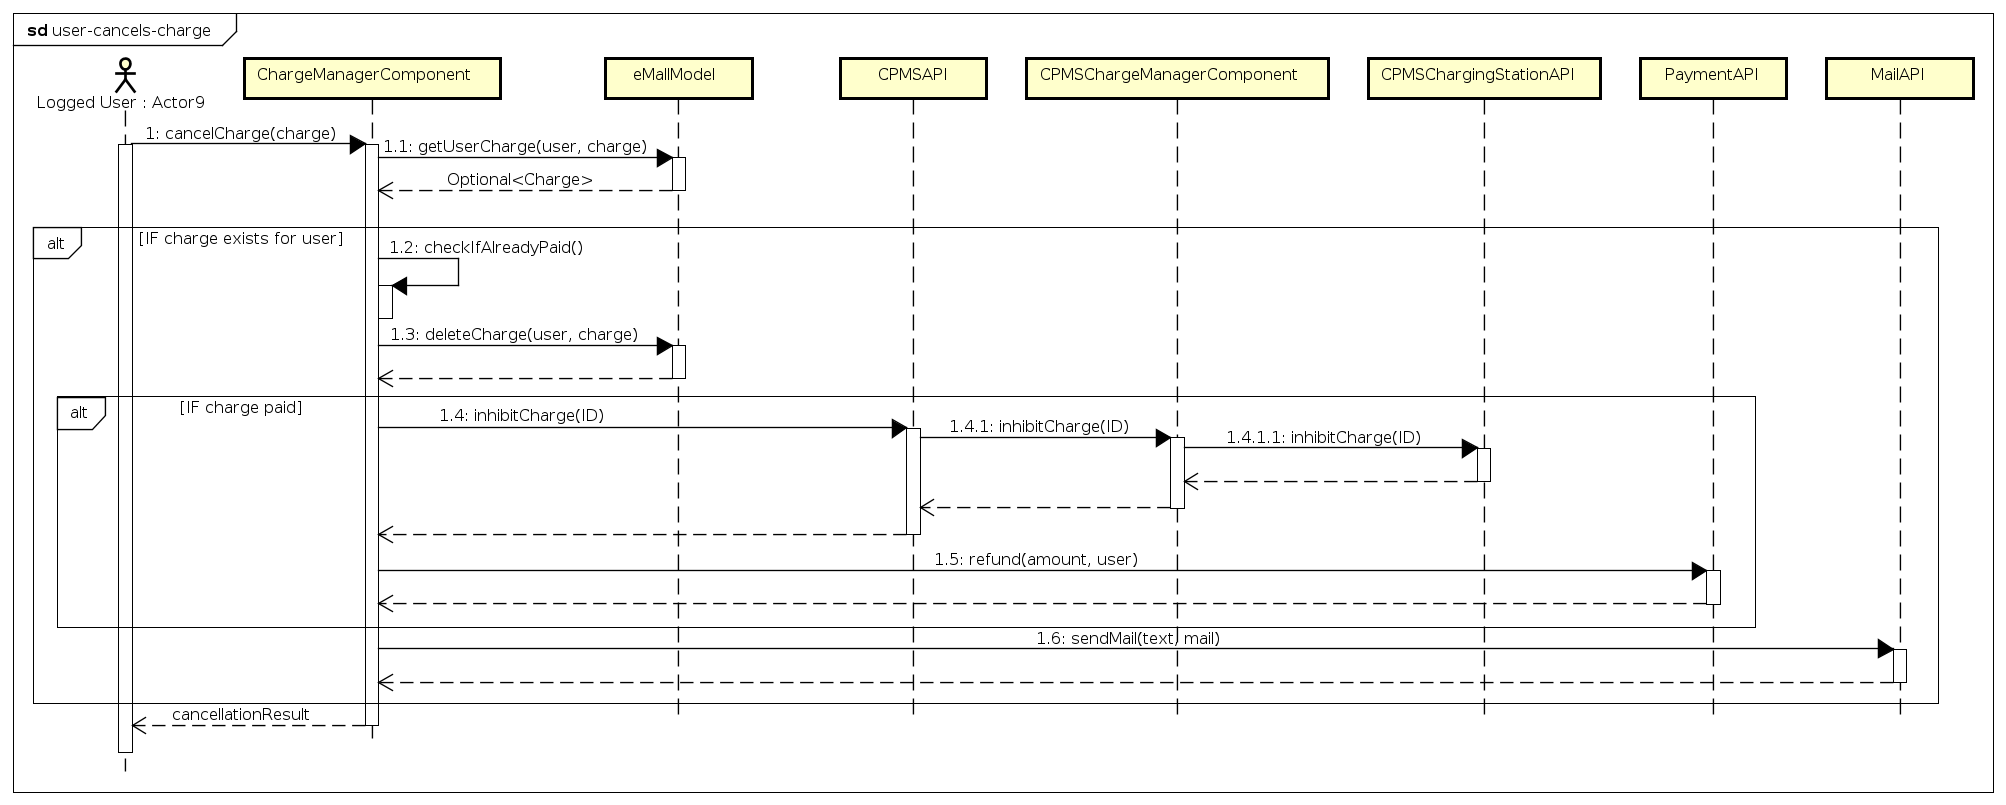
\includegraphics[keepaspectratio, width=16cm]{Sequence/user-cancels-charge.png}
        \caption{Cancel a charge sequence}
        \label{fig:user-cancels-charge}
    \end{center}
\end{figure}
\begin{figure}[!h]
    \begin{center}
        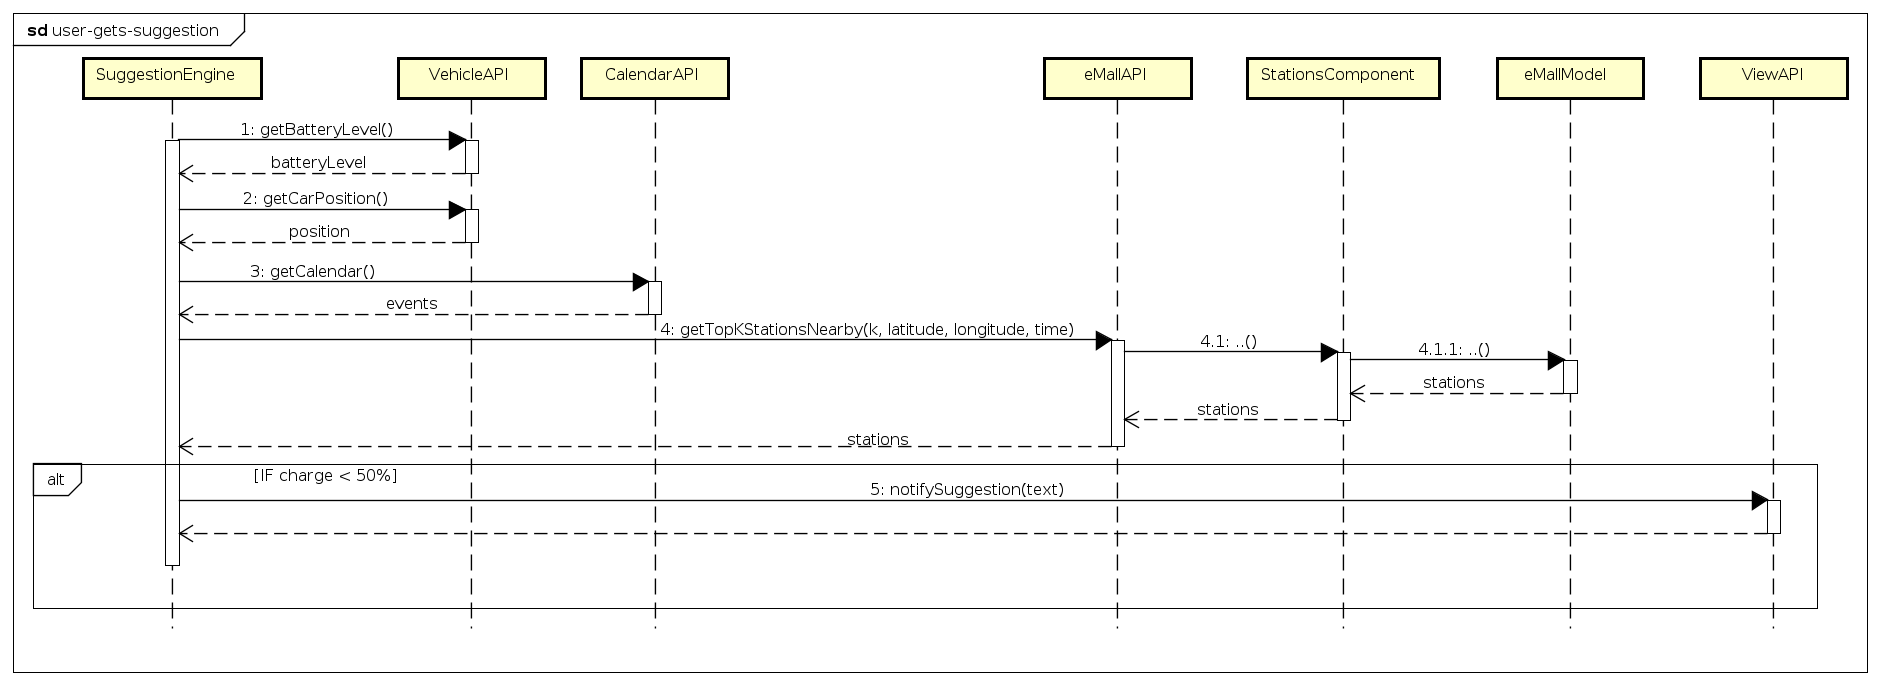
\includegraphics[keepaspectratio, width=16cm]{Sequence/user-gets-suggestion.png}
        \caption{Get a suggestion sequence}
        \label{fig:user-gets-suggestion}
    \end{center}
\end{figure}
\begin{figure}[!h]
    \begin{center}
        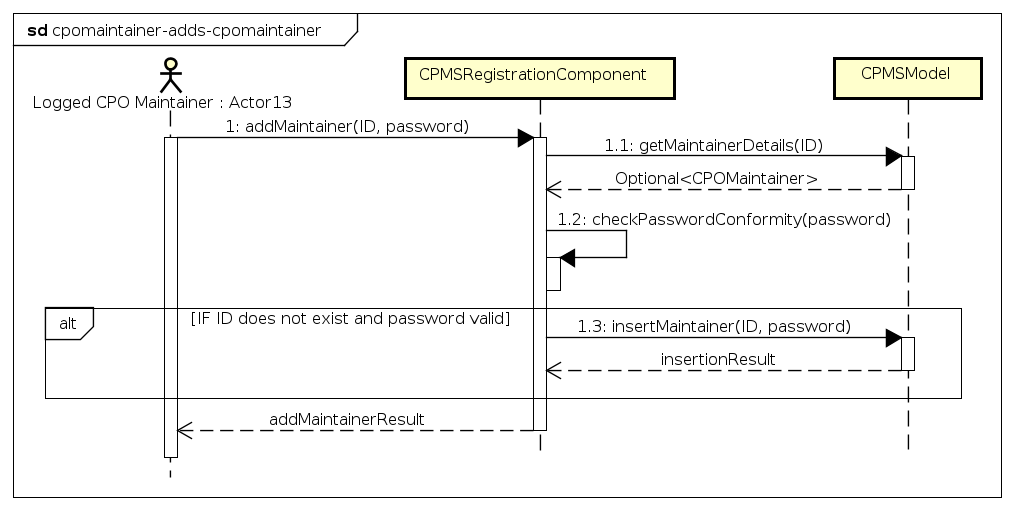
\includegraphics[keepaspectratio, width=16cm]{Sequence/cpomaintainer-adds-cpomaintainer.png}
        \caption{\ac{CPO}maintainer adds \ac{CPO}maintainer to \ac{CPMS}}
        \label{fig:cpomaintainer-adds-cpomaintainer}
    \end{center}
\end{figure}
\begin{figure}[!h]
    \begin{center}
        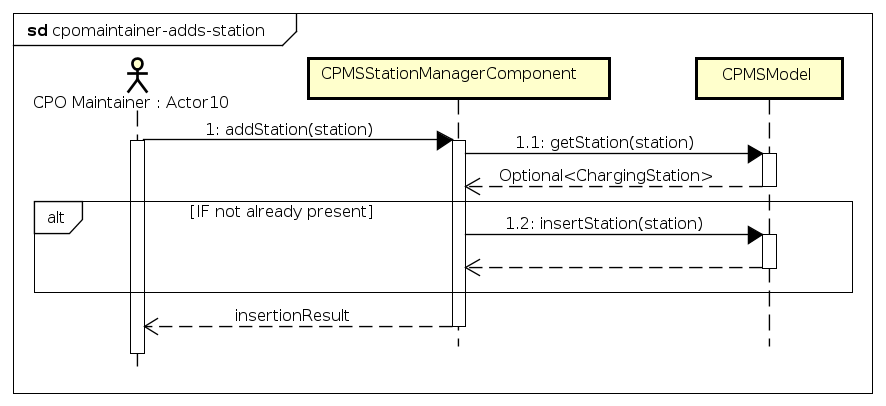
\includegraphics[keepaspectratio, width=16cm]{Sequence/cpomaintainer-adds-stations.png}
        \caption{\ac{CPO}maintainer adds stations to \ac{CPMS}}
        \label{fig:cpomaintainer-adds-stations}
    \end{center}
\end{figure}
\begin{figure}[!h]
    \begin{center}
        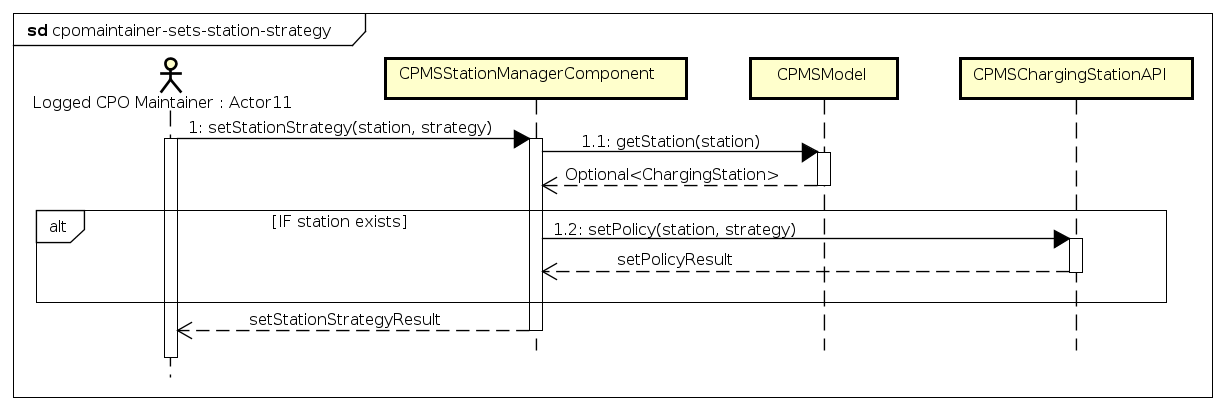
\includegraphics[keepaspectratio, width=16cm]{Sequence/cpomaintainer-sets-station-strategy.png}
        \caption{\ac{CPO}maintainer sets station strategy in \ac{CPMS}}
        \label{fig:cpomaintainer-sets-station-strategy}
    \end{center}
\end{figure}
\begin{figure}[!h]
    \begin{center}
        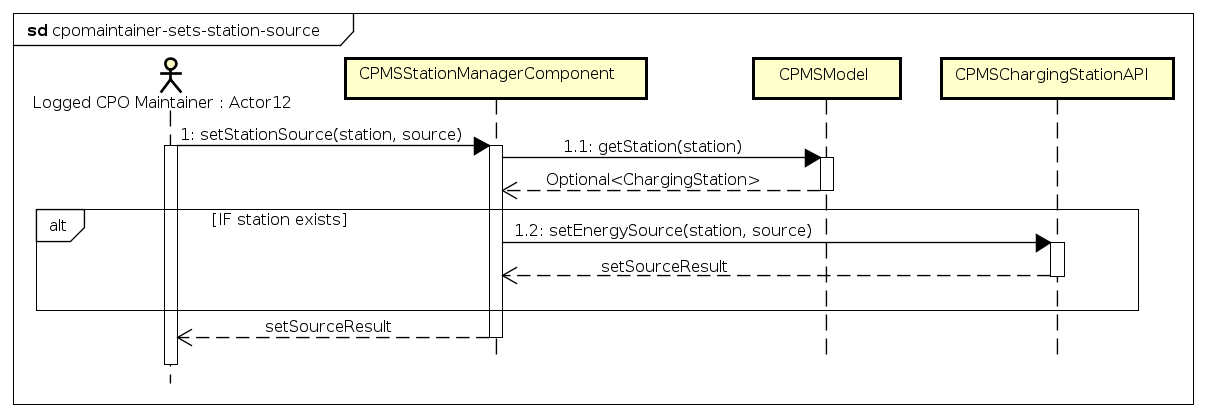
\includegraphics[keepaspectratio, width=16cm]{Sequence/cpomaintainer-sets-station-source.png}
        \caption{\ac{CPO}maintainer sets station source in \ac{CPMS}}
        \label{fig:cpomaintainer-sets-station-source}
    \end{center}
\end{figure}
\clearpage
There are some particular design decisions that need to be clarified:
\begin{itemize}
    \item \textbf{Login sequences:} In \autoref{fig:user-executes-authorized-command} and \autoref{fig:cpomaintainer-executes-authorized-command} it is illustrated the way the system authorizes \acp{CPO} and users. It filters authorized commands using functions (like \cite{ref:command-pattern}). The component that filters the requests is the AuthorizationComponent (present in both \ac{eMall} and \ac{CPMS} systems).\\
          When the client utilizes the interface, automatically it has to send also his credentials; these are then verified by the AuthorizationComponent and, if correct it executes the corresponding \ac{API} function. This pattern allows the system to decentralize the authorization verification from the \ac{API} code and allows every function that needs this data to have access to the client's account information;
    \item \textbf{Asynchronous messages:} During the inter-system communications (like \ac{eMall} -> \ac{CPMS} or \ac{CPMS} -> ChargingStation) it would be useful to implement asynchronous communications to avoid blocking situations. However in the sequence diagrams there aren't any because a better solution (compromise between having a completely asynchronous communication and having feedback from the interface) is to implement a timeout timer to avoid a deadlock. This information is not shown in the sequence diagrams due to its verbosity of notation.

\end{itemize}
\clearpage
\subsection{Component interfaces}
\begin{figure}[!h]
    \begin{center}
        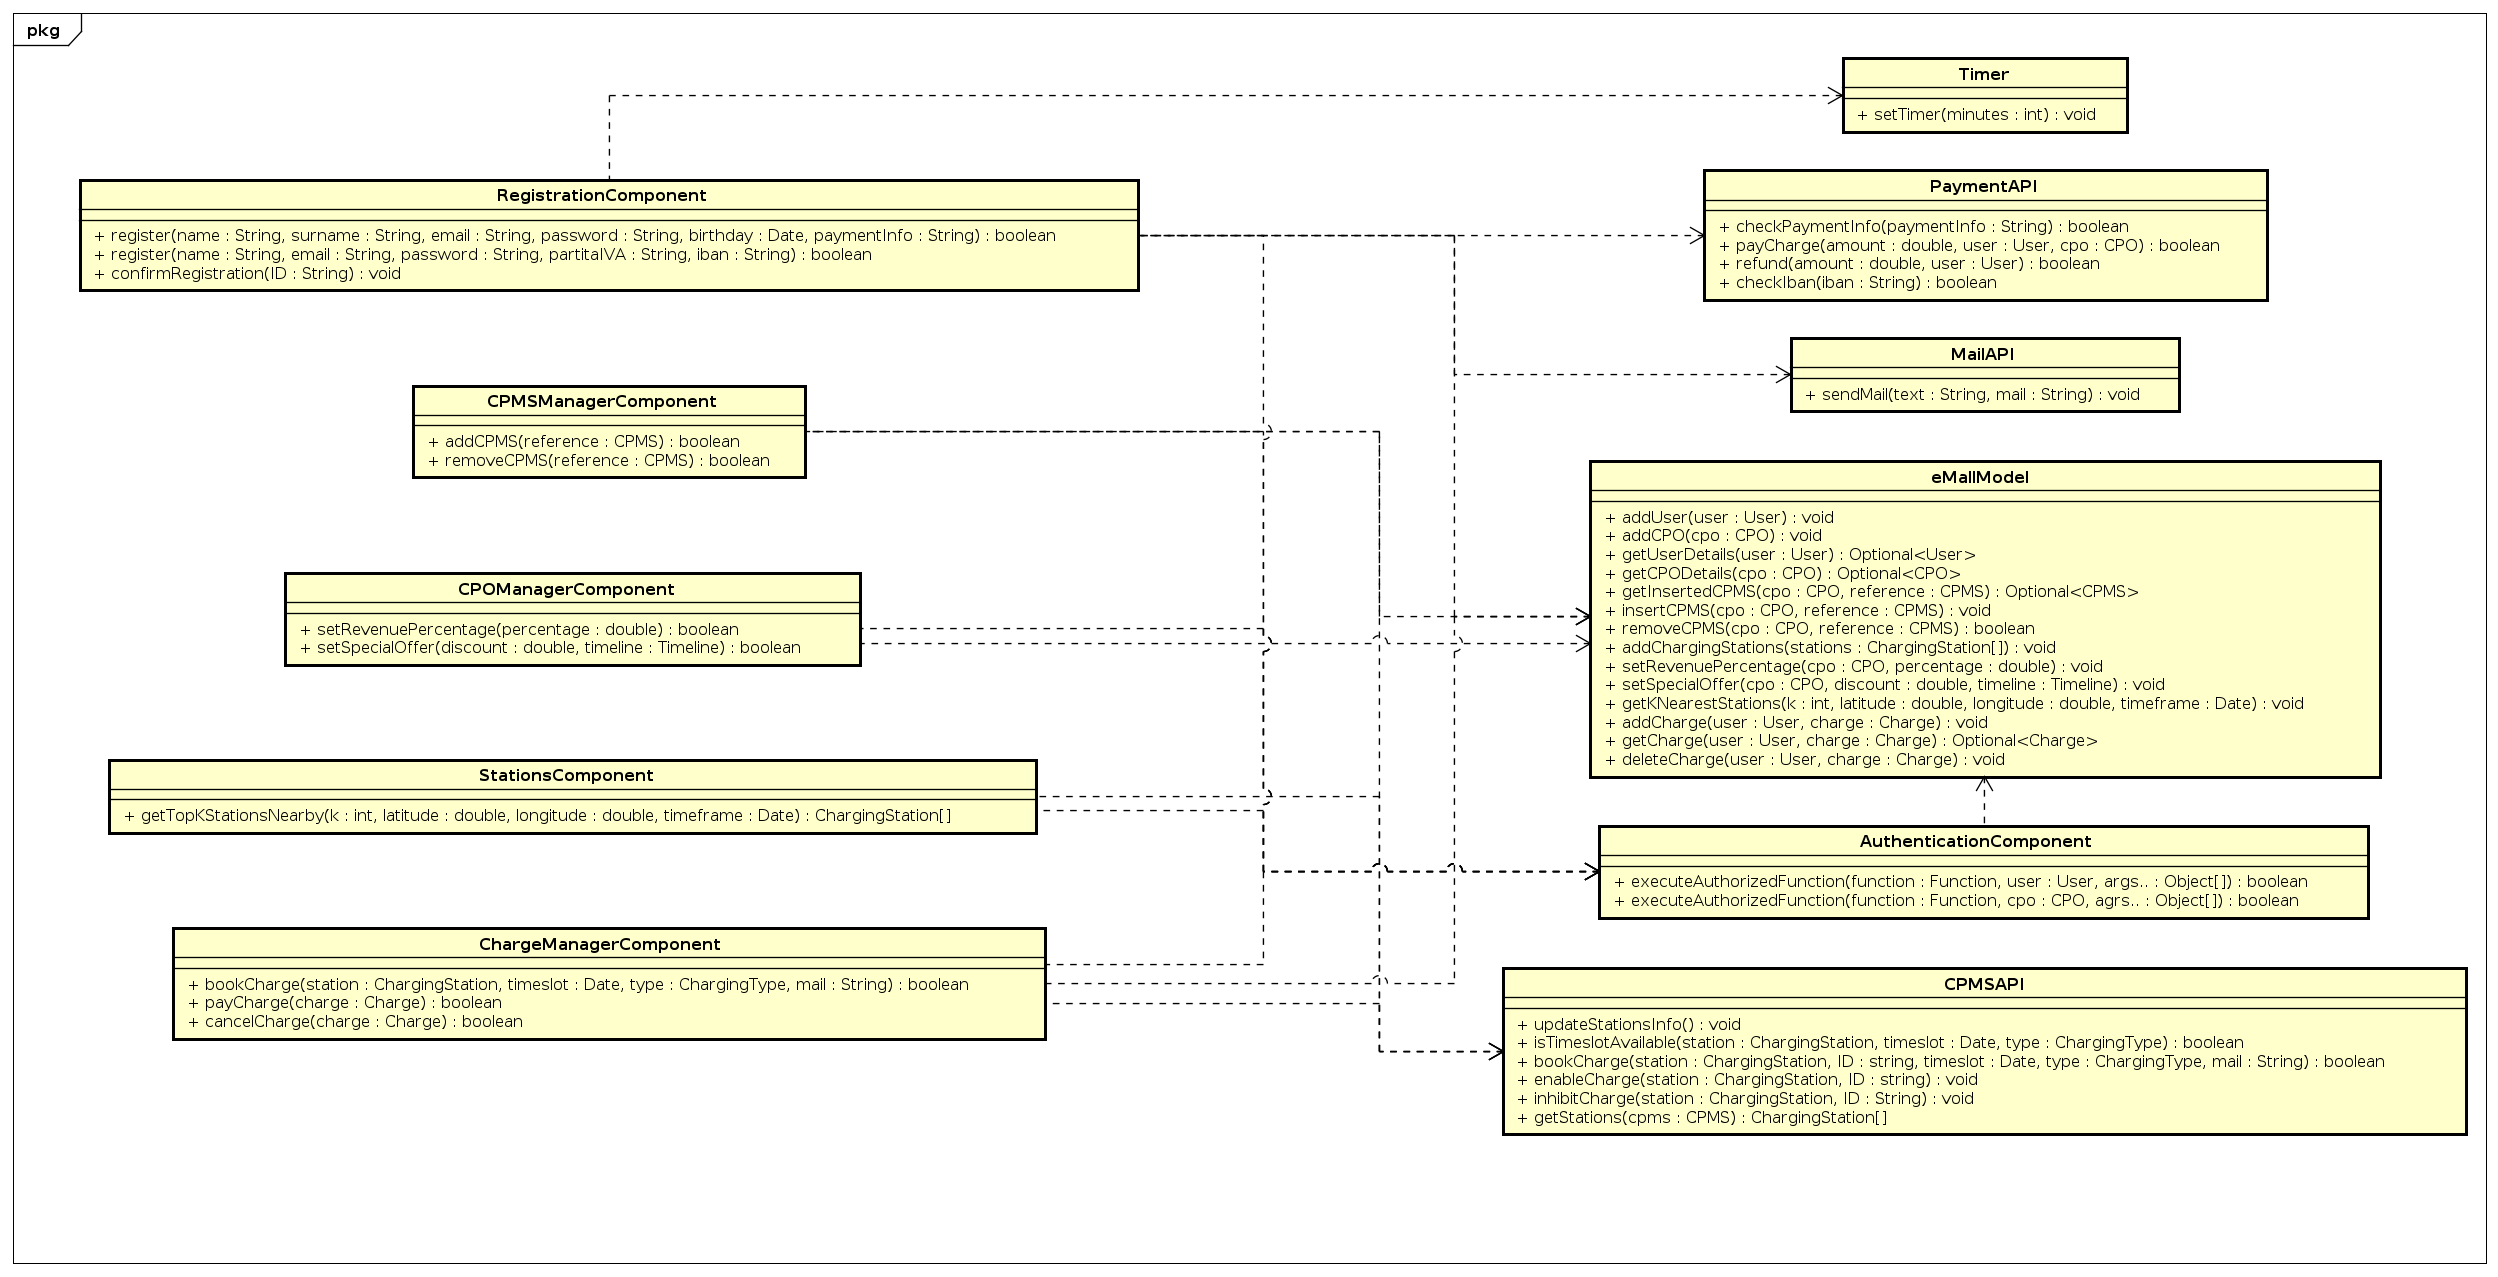
\includegraphics[keepaspectratio, width=16cm]{Interface/eMallInterface.png}
        \caption{\ac{eMall} components interface}
        \label{fig:emall-interface}
    \end{center}
\end{figure}
\begin{figure}[!h]
    \begin{center}
        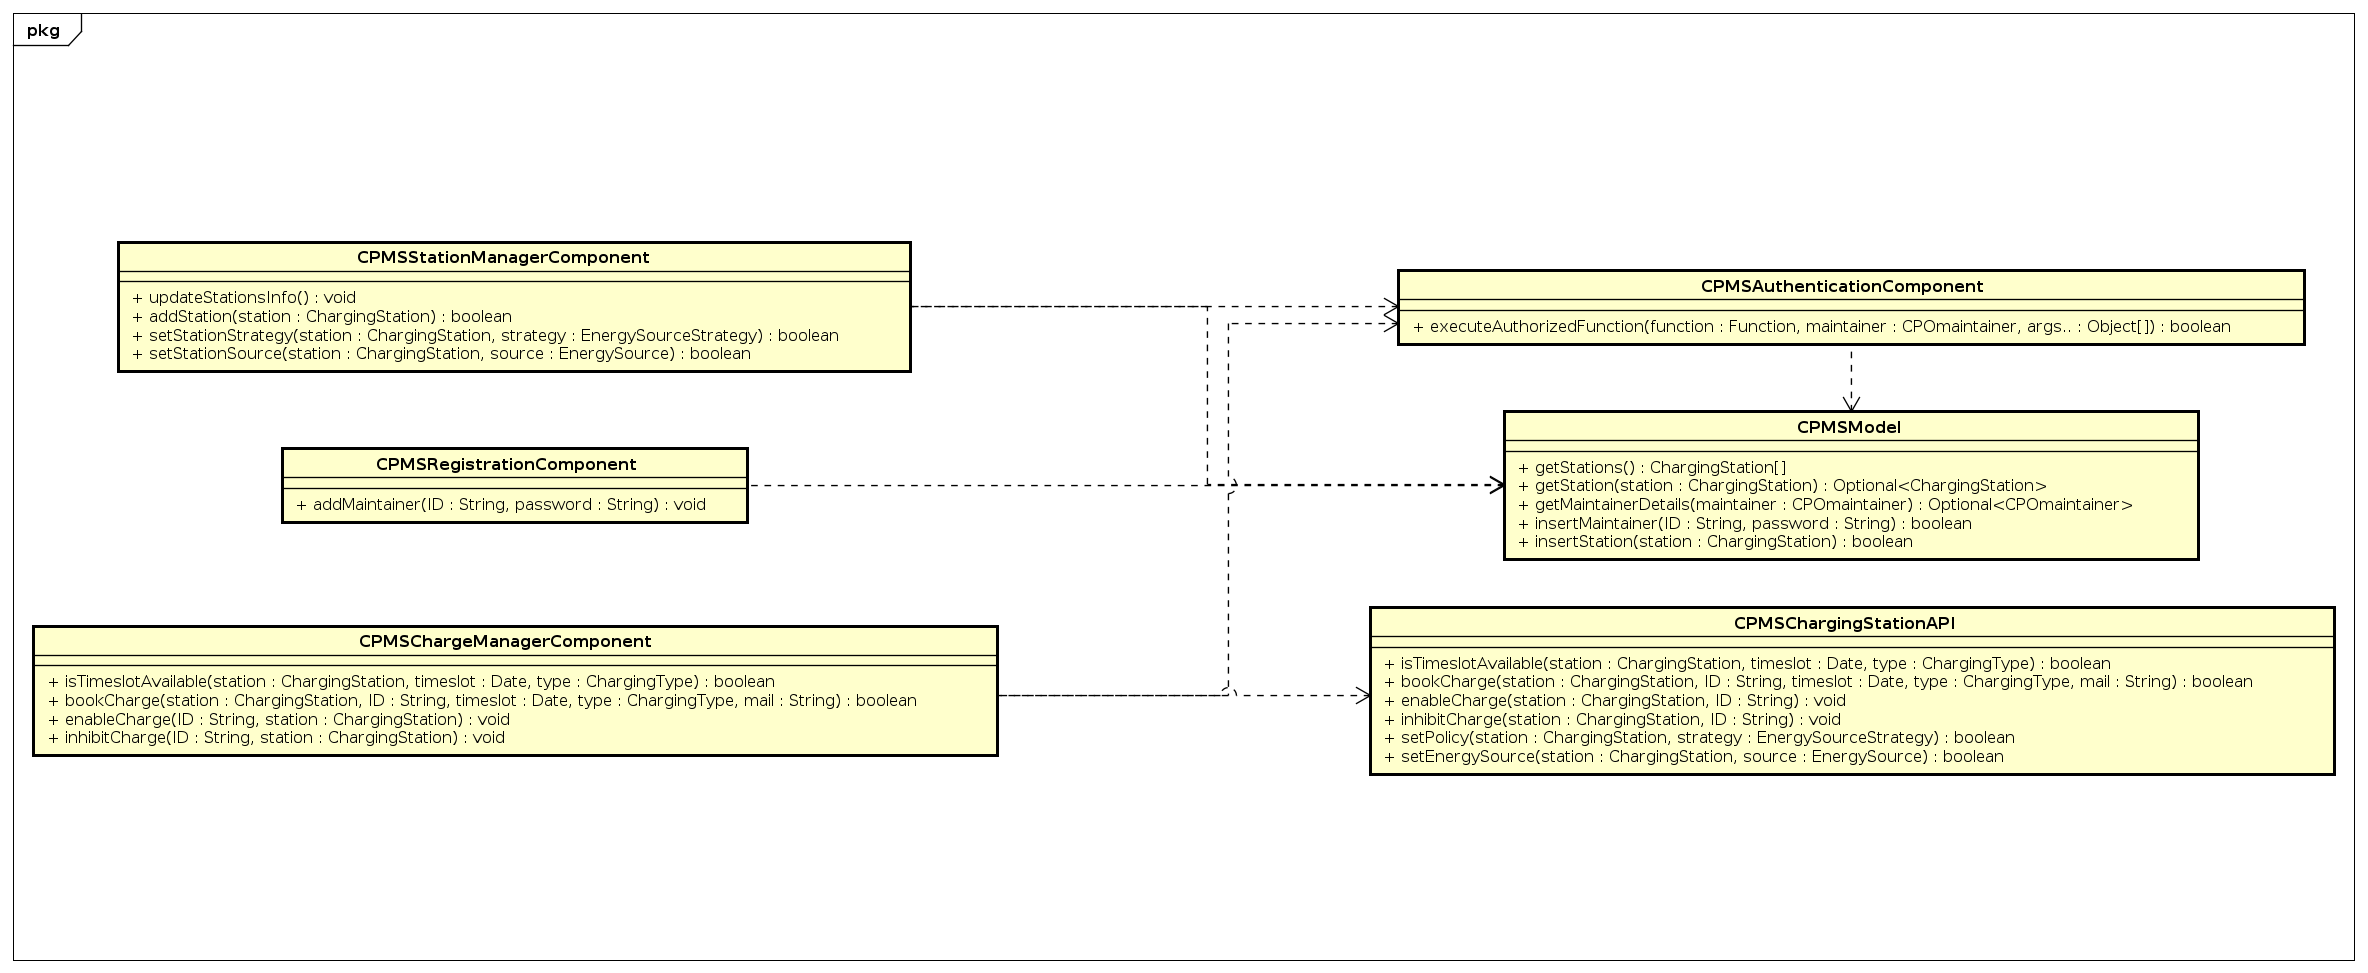
\includegraphics[keepaspectratio, width=16cm]{Interface/CPMSInterface.png}
        \caption{\ac{CPMS} components interface}
        \label{fig:cpms-interface}
    \end{center}
\end{figure}
The \ac{eMall} client interface diagram is not present due to the absence of concrete exposed interfaces. Here follows a brief clarification about the client components' interactions:
\begin{itemize}
    \item \textbf{Vehicle and Calendar \acp{API}:} allow the local system to interface itself with the car and the user's calendar if any. They both serve the SuggestionEngine component which is a thread that continues checking the need of a recharge;
    \item \textbf{\ac{eMall} \ac{API}:} allows the client to interact with the business logic layer of the system. It is interrogated by the suggestion engine and the view component;
    \item \textbf{\ac{eMall}ViewComponent:} interacts with the suggestion engine and the \ac{eMall} \ac{API} to visualize the application (it is the view in \ac{MVC} pattern).
\end{itemize}
The main aspect that makes this subsystem a fat client is that the SuggestionEngine continues interrogating the eMall, the vehicle and the calendar \acp{API} in order to proactively suggest a charge to the user.

\subsection{Selected architectural styles and patterns}
\begin{itemize}
    \item Bridge pattern \cite{ref:bridge-pattern}: It consists in decoupling completely two systems by having two interfaces. In \autoref{fig:bridge-pattern} there is a simplification of the architecture in order to highlight the usage of this pattern.
          Instead of having a complex system with the composition of an \ac{eMSP} and a \ac{CPMS} we exploit their interfaces in order to implement them in a decoupled way. The \ac{eMSP} implementation (i.e. \ac{eMall}) interacts with a \ac{CPMS} interface. This pattern allows an implementation-independent interface. \label{pattern:bridge}
\end{itemize}

\begin{figure}[!h]
    \begin{center}
        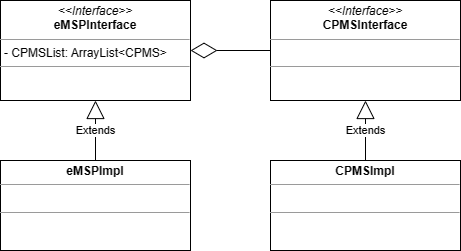
\includegraphics[keepaspectratio, width=12cm]{Graphics/DD-bridge-pattern.drawio.png}
        \caption{Bridge pattern representation in the system}
        \label{fig:bridge-pattern}
    \end{center}
\end{figure}

\subsubsection{\ac{eMSP} architectural styles and patterns}
\begin{itemize}
    \item \acl{MVC} pattern \cite{ref:MVC-pattern}: It consists in grouping the system in three clusters:
          \begin{itemize}
              \item the model, with all the persistent data of the system;
              \item the view, with the logic to present the model;
              \item the controller, with the business logic for elaborating requests from the view and manipulating the model.
          \end{itemize}
          The controller component is then divided into two classes:
          the first, distributed on the client, elaborates the data retrieved from the calendar and the vehicle in order to avoid cumbersome requests to the server;
          the second, distributed on the application server, handles the requests made by the client and interacts with the model.
    \item The three-tier architecture \cite{ref:multitier-pattern}: It increases the modularity and manageability of the system by dividing it into presentation, application, and data tiers. This allows for improving a single tier without affecting the others.
    \item The \ac{DAO} pattern \cite{ref:dao-pattern}: It maps relational database tables directly to objects in the application. This decouples the application and data layers further.
\end{itemize}

\subsubsection{\ac{CPMS} architectural styles and patterns}
\begin{itemize}
    \item The \acl{MVC} pattern \cite{ref:MVC-pattern}: is used to decouple the view logic from the rest of the system, simplify code organization and implementation, and provide a software layer to handle access to the model and prevent the presentation layer from directly accessing the model.
    \item The two-tier architecture \cite{ref:multitier-pattern} is used because the \ac{CPMS} does not need to handle as much traffic as an \ac{eMSP} system. As a result, it is simpler and only has two tiers: a thin-client with the presentation layer, which handles the view logic, and an application server.
\end{itemize}


\subsection{Other design decisions}
\subsubsection{\ac{SPOF} avoidance}
Both the \ac{eMSP} and \ac{CPMS} systems have been designed with a focus on avoiding \acp{SPOF}. As \ac{eMall} is a large service that competes with other similar services, this quality can also be a competitive advantage. In addition, with many potential users accessing the service at the same time, a downtime would result in a significant loss of money and damage to the public image. The cost of having and maintaining a redundant system is justified by the increased availability of the system.
These decisions can be seen in Figures \autoref{fig:eMSP-deployment} and \autoref{fig:CPMS-deployment}.
\paragraph{Firewalls, load balancers, \ac{VPN} servers}
For firewalls \cite{ref:redundant-firewalls}, load balancers \cite{ref:redundant-load-balancers}, and \ac{VPN} servers \cite{ref:redundant-VPN-servers}, the general pattern is to have a floating IP \cite{ref:floating-ip} mapped to the exposed service, and two physical redundant systems that are directly connected to send and receive a "heartbeat" signal indicating that the system is up and running. If one system does not receive the heartbeat from the other, the floating IP linked to the service is redirected to the active system.
\paragraph{Application server}
For the application server, we use the load balancers to use both application servers (if available) or just the active one if the other is unavailable.
\paragraph{Databases}
The database system is designed to withstand temporary failures of a database server and to be able to recover from disasters. A secondary database server is synchronized in real-time to take over if the primary database server goes down. A third database server is located in a different location from the other two to enable a disaster-recovery plan; this server is synchronized once a day.
\clearpage